% MISO-TFA simulation and NC validation manuscript draft.
% Figures and exact numerical macros are generated by
% miso_tfa/modules/reporting/generateManuscriptAssets.m.

\documentclass[12pt]{article}

\usepackage[T1]{fontenc}
\usepackage[utf8]{inputenc}
\usepackage[margin=1in]{geometry}
\usepackage{amsmath,amssymb}
\usepackage{graphicx}
\usepackage{booktabs}
\usepackage{longtable}
\usepackage{array}
\usepackage{tabularx}
\usepackage{caption}
\usepackage{subcaption}
\usepackage{float}
\usepackage{xcolor}
\usepackage{hyperref}
\usepackage{enumitem}
\usepackage{setspace}

\hypersetup{
    colorlinks=true,
    linkcolor=blue!55!black,
    citecolor=blue!55!black,
    urlcolor=blue!55!black
}

\graphicspath{{figures/}}
\setstretch{1.25}
\setlength{\parindent}{0.3in}
\setlength{\parskip}{0.15em}
\setcounter{secnumdepth}{3}

\newcommand{\MAP}{\mathrm{MAP}}
\newcommand{\COtwo}{\mathrm{CO_2}}
\newcommand{\CBFV}{\mathrm{CBFV}}
\newcommand{\MISO}{\mathrm{MISO}}
\newcommand{\SISO}{\mathrm{SISO}}
\newcommand{\Advantage}{\mathrm{Advantage}}

\IfFileExists{tables/results_values.tex}{% Generated by generateManuscriptAssets.m.
\newcommand{\SimulationTotalAnalyses}{52000}
\newcommand{\SimulationBootstrapSamples}{2000}
\newcommand{\MaximumMonteCarloSE}{0.0310}
\newcommand{\PrimaryPrecisionPassRate}{100.0\%}
\newcommand{\NCSubjectCount}{23}
\newcommand{\NCAdvantageMinimum}{-0.440}
\newcommand{\NCAdvantageMaximum}{-0.077}
\newcommand{\NCFrequencyCount}{30}
\newcommand{\NCNegativeCount}{30}
\newcommand{\NCBelowZeroCount}{26}
\newcommand{\NCIncludesZeroCount}{4}
}{}

\title{When does modeling MAP and carbon dioxide together improve cerebral\
hemodynamic transfer-function estimates? A known-truth simulation and\
held-out normal-control study}
\author{[Author names and affiliations to be added]}
\date{Simulation study manuscript draft -- \today}

\begin{document}

\maketitle

\begin{abstract}
\textbf{Background:} Transfer function analysis describes how fluctuations in
arterial pressure are reflected in cerebral blood flow velocity (CBFV) at
different frequencies. Carbon dioxide is another strong regulator of cerebral
vascular tone. When mean arterial pressure (MAP) and carbon dioxide change
together, a MAP-only estimate can contain information associated with both
inputs.

\textbf{Objective:} We designed a reproducible simulation study to identify
when a two-input, single-output (MISO) model recovers the separate MAP-to-CBFV
and carbon-dioxide-to-CBFV pathways more accurately than separate
single-input, single-output (SISO) models. We then applied the same blocked
comparison to normal-control (NC) recordings, where the true human pathways
are unknown.

\textbf{Methods:} At 4~Hz, MAP and carbon dioxide signals were generated with
controlled frequency content and controlled dependence, passed through known
pathways, and combined to form CBFV. The primary design varied input
coherence, relative carbon-dioxide pathway strength, recording duration, and
CBFV output signal-to-noise ratio. Timing, MAP and carbon-dioxide recording
noise, alignment error, and output-noise shape were examined as sensitivity
conditions. The endpoint was the frequency-specific log ratio of SISO error to
MISO error; positive values favor MISO. Production used 500 paired families per
condition and 2,000 paired bootstrap draws. NC validation used disjoint
recording blocks and subject bootstrap.

\textbf{Results:} The production study contained \SimulationTotalAnalyses{}
analyses. All finite primary-map cells met the predeclared Monte Carlo
standard-error target, with a worst standard error of
\MaximumMonteCarloSE{} log$_{10}$ units. MISO advantage varied with frequency,
input dependence, pathway balance, recording duration, and output noise. The
NC held-out prediction curve ranged from \NCAdvantageMinimum{} to
\NCAdvantageMaximum{} across the retained frequency grid. Because all of
these values were negative, the NC prediction comparison did not show a
held-out MISO advantage over the paired SISO comparator in this analysis.

\textbf{Conclusion:} The simulation separates two questions that are often
combined: whether MISO can recover a known pathway more accurately, and whether
it predicts a held-out human recording better. The results provide operating
conditions under which the extra MISO pathway is useful, as well as conditions
under which the simpler SISO estimate is adequate or preferable.
\end{abstract}

\noindent\textbf{Keywords:} cerebral hemodynamics; transfer function analysis;
MISO; SISO; carbon dioxide; cerebral blood flow velocity; simulation study;
bootstrap validation

\newpage
\tableofcontents
\newpage

\section{Introduction}

The brain requires continuous blood flow while arterial pressure changes from
moment to moment. Cerebral autoregulation helps limit the effect of these
pressure changes on cerebral perfusion. Dynamic cerebral autoregulation focuses
on how this response develops over time. It is commonly assessed using mean
arterial pressure (MAP) and cerebral blood flow velocity (CBFV), measured with
transcranial Doppler. CBFV is used as a surrogate for changes in flow when the
diameter of the insonated artery is sufficiently stable \cite{Panerai2023}.

Transfer function analysis (TFA) describes the relationship between these
signals across frequency. A recording contains fluctuations that occur over
different timescales: a fluctuation at 0.10~Hz repeats once every 10 seconds,
whereas one at 0.20~Hz repeats once every 5 seconds. TFA asks how the size and
timing of CBFV fluctuations relate to MAP fluctuations at each of these
frequencies. This matters because the cerebral circulation may respond
differently to slower and faster pressure changes.

The transfer function summarizes two properties. Gain describes the size of
the CBFV response relative to the MAP fluctuation. Phase describes their
relative timing as a fraction of a cycle, expressed in degrees or radians.
For example, a one-second timing difference spans one-tenth of a cycle, or
36 degrees, at 0.10~Hz. Gain and phase are stored together in a complex-valued
transfer function; the complex notation retains both response size and timing
in one quantity. Coherence is calculated alongside it and describes the
strength of the linear relationship between the signals at each frequency.
These measures describe the observed pressure--velocity relationship, whose
interpretation also depends on other influences on CBFV \cite{Panerai2023}.

\subsection{Why MAP-only analysis can mix inputs}

Most pressure--flow analyses use a single-input, single-output (SISO) model,
with MAP as the input and CBFV as the output. This model describes their
pairwise relationship. Interpreting it as a separate pressure-related response
requires considering whether another influence on CBFV also varies with MAP.

Carbon dioxide is one such influence. Changes in arterial CO$_2$ alter
cerebrovascular tone, with increasing CO$_2$ generally increasing cerebral
blood flow and decreasing CO$_2$ reducing it \cite{Hoiland2019}. In resting
recordings, end-tidal CO$_2$ provides a practical breath-to-breath surrogate
for arterial CO$_2$, although the two measurements are not interchangeable.
We use CO$_2$ as shorthand for this measured end-tidal signal in the human
analysis and for the corresponding input in the simulation.

Suppose MAP and CO$_2$ tend to rise together and both contribute to a rise in
CBFV. A MAP-only model cannot determine from that pair alone how much of the
CBFV change was associated with CO$_2$. It may therefore attribute some of
the CO$_2$ response to MAP. The same issue applies in reverse to a CO$_2$-only
model. Two separate SISO analyses retain useful pairwise descriptions, but
neither explicitly accounts for the other measured input. A change in apparent
MAP responsiveness could therefore reflect altered CO$_2$ dynamics as well as
altered pressure regulation.

The relevant relationship is MAP--CO$_2$ \emph{input coherence}, which
describes their linear dependence at each frequency. Its population value
ranges from zero for no linear relationship to one for a perfect linear
relationship. It is different from MAP--CBFV or CO$_2$--CBFV coherence.
Two signals can both contain fluctuations at the same frequency but have low
coherence if their relative timing or amplitude changes from one recording
segment to another. Coherence is high only when that relationship remains
consistent. Their relative phase, together with the two pathway responses,
determines how their CBFV contributions combine. Omitting CO$_2$ can therefore
change the apparent MAP gain, phase, or both, and need not always increase the
apparent response.

\subsection{What the two-input model changes}

A multiple-input, single-output (MISO) model includes MAP and CO$_2$ in one
joint analysis of CBFV. It estimates the MAP response while accounting for
CO$_2$, and the CO$_2$ response while accounting for MAP. These are called
conditional responses because each estimate depends on which other input is
included. Here, a pathway means the frequency-specific relationship assigned
to one input in this model. It is a model-defined response component, not an
independently measured anatomical or causal pathway in human recordings.

The two-input model represents the CBFV fluctuation at frequency $f$ as the
sum of a MAP-related contribution, a CO$_2$-related contribution, and a
remaining unexplained component:

\begin{equation}
    Y(f) = H_M(f)M(f) + H_C(f)C(f) + E(f),
    \label{eq:conceptual_generator}
\end{equation}

Here, $M$, $C$, and $Y$ represent MAP, CO$_2$, and CBFV fluctuations at that
frequency. Multiplying $M$ by its transfer function $H_M$ changes its amplitude
and phase to give the MAP-related CBFV contribution; $H_C C$ does the same for
CO$_2$. The term $E$ contains the CBFV fluctuation left unexplained by the two
inputs. The model assumes that these contributions add and that their response
properties remain sufficiently stable over the analyzed recording. MISO uses
the relationship between MAP and CO$_2$, as well as each input's relationship
with CBFV, to estimate $H_M$ and $H_C$ together. Recovering the two responses
requires MAP and CO$_2$ to contain some frequency-specific variation that is
not shared. This does not require the inputs to be completely independent, but
if they are nearly identical at a frequency, the model cannot reliably assign
the observed CBFV fluctuation to one input or the other. The unexplained
component must also lack a systematic relationship with either input;
otherwise, input-related variation omitted from the model can be absorbed into
the estimated responses. Adding CO$_2$ alone does not account for every other
influence on CBFV.

Previous studies provide a physiological basis for this approach. Panerai and
colleagues modeled spontaneous pressure and end-tidal CO$_2$ fluctuations
together and found that adding CO$_2$ reduced the error in describing resting
CBFV \cite{Panerai2000}. Their error was the mean squared difference between
measured CBFV and the CBFV reconstructed by the model. It therefore measured
overall reconstruction rather than recovery of the individual MAP and CO$_2$
transfer functions. Peng and colleagues included pressure, end-tidal
CO$_2$, and end-tidal oxygen, finding higher multiple coherence below 0.05~Hz
than with pressure alone \cite{Peng2008}. Multiple coherence describes how
much of the output's frequency-specific variation is represented by all
included inputs together. These findings establish the relevance of additional
inputs, while leaving a separate question: how accurately are their individual
transfer functions estimated?

There are two potential benefits to including CO$_2$. First, when MAP and
CO$_2$ vary together, MISO can reduce systematic mixing of their responses.
Second, even when the inputs are independent, CO$_2$ can explain CBFV
fluctuations that remain in the residual of a MAP-only model. In an infinitely
long recording, these fluctuations would not systematically bias the MAP-only
estimate, but in a finite recording they can make that estimate more variable.
Fitting a separate CO$_2$ SISO model does not remove this variation from the
MAP fit because each SISO model is estimated without accounting for the other
input. By estimating both responses together, MISO can reduce this source of
finite-record variability. The first potential benefit concerns systematic
error, or bias; the second concerns variability between estimates. Low input
coherence therefore does not, by itself, imply that including CO$_2$ has no
value.

These potential benefits must be balanced against estimating two responses
from a finite recording. If the CO$_2$ contribution is negligible, the added
pathway may provide little benefit. If MAP and CO$_2$ are nearly linearly
dependent at a frequency, many combinations of their estimated responses can
produce a similar CBFV fluctuation, making the separate estimates sensitive to
small recording errors. This difficulty also arises in other physiological
systems with strongly coupled inputs \cite{Westwick2006}. Short recordings,
measurement noise, and signal misalignment can further limit accuracy. Whether
MISO improves an estimate therefore depends on both the underlying
relationships and the information available in the recording.

\subsection{Why a known-truth simulation is needed}

Human recordings provide measured inputs and CBFV, but the true individual
transfer functions are unknown. A difference between SISO and MISO estimates
therefore cannot establish which is closer to the underlying response.
Likewise, explaining more CBFV variation in the recording used to fit a model
does not establish accurate separation: errors in the two estimated pathways
can partly compensate for one another in their combined output.

A known-truth simulation makes pathway accuracy directly testable. The MAP
and CO$_2$ transfer functions are specified first. Generated inputs are passed
through those functions and their contributions are combined to form CBFV.
SISO and MISO receive the same observed signals, without access to the
generating functions. Their estimated gain and phase can then be compared
with the known responses. Both methods are judged against the individual
generating pathway: the question is how well a pairwise SISO estimate or a
conditional MISO estimate approximates that target. Repeating the procedure
with different random signals measures variability between estimates.

Known-system simulations have also been used to evaluate cerebral
autoregulation methods. Chertoff and colleagues tested recovery of specified
linear and nonlinear responses before applying their method to human
recordings \cite{Chertoff2020}. Here, the same validation principle is applied
to the simpler question of separating two linear input pathways.

This is a controlled test of recovery when a linear two-input model is the
generating system. It does not assume that human cerebrovascular regulation
is fully described by two inputs. Testing an absent or weak CO$_2$ contribution,
as well as noisy and strongly dependent inputs, allows the comparison to
identify conditions in which estimating the additional pathway is unnecessary
or unreliable. Both methods use the same observations and spectral-estimation
settings under each declared condition.

\subsection{Study objective}

The primary objective was to determine when MISO more accurately recovers the
separate MAP-to-CBFV and CO$_2$-to-CBFV transfer functions than the corresponding
SISO analyses. We examined input dependence, relative CO$_2$ pathway strength,
recording duration, and CBFV output noise, with additional tests of input
recording noise and timing. The main displays vary one quantity at a time
around a declared reference condition. Frequency is retained on the horizontal
axis, the tested quantity on the vertical axis, and relative MISO accuracy in
the color scale, so that benefits at one frequency are not hidden by averaging
across the entire band.

Normal-control (NC) recordings informed selected properties of the simulated
inputs and provided a separate test of CBFV prediction. For that test, models
were estimated from part of each recording and used to predict CBFV in a
held-out part that was not used for estimation. This evaluates prediction on
unseen data, while the simulation evaluates recovery of known pathways.
Together, these analyses support a reproducible workflow for applying SISO
and MISO to measured MAP, CO$_2$, and CBFV signals and for assessing how
recording conditions affect their accuracy
(Figure~\ref{fig:design}).

\begin{figure}[H]
    \centering
    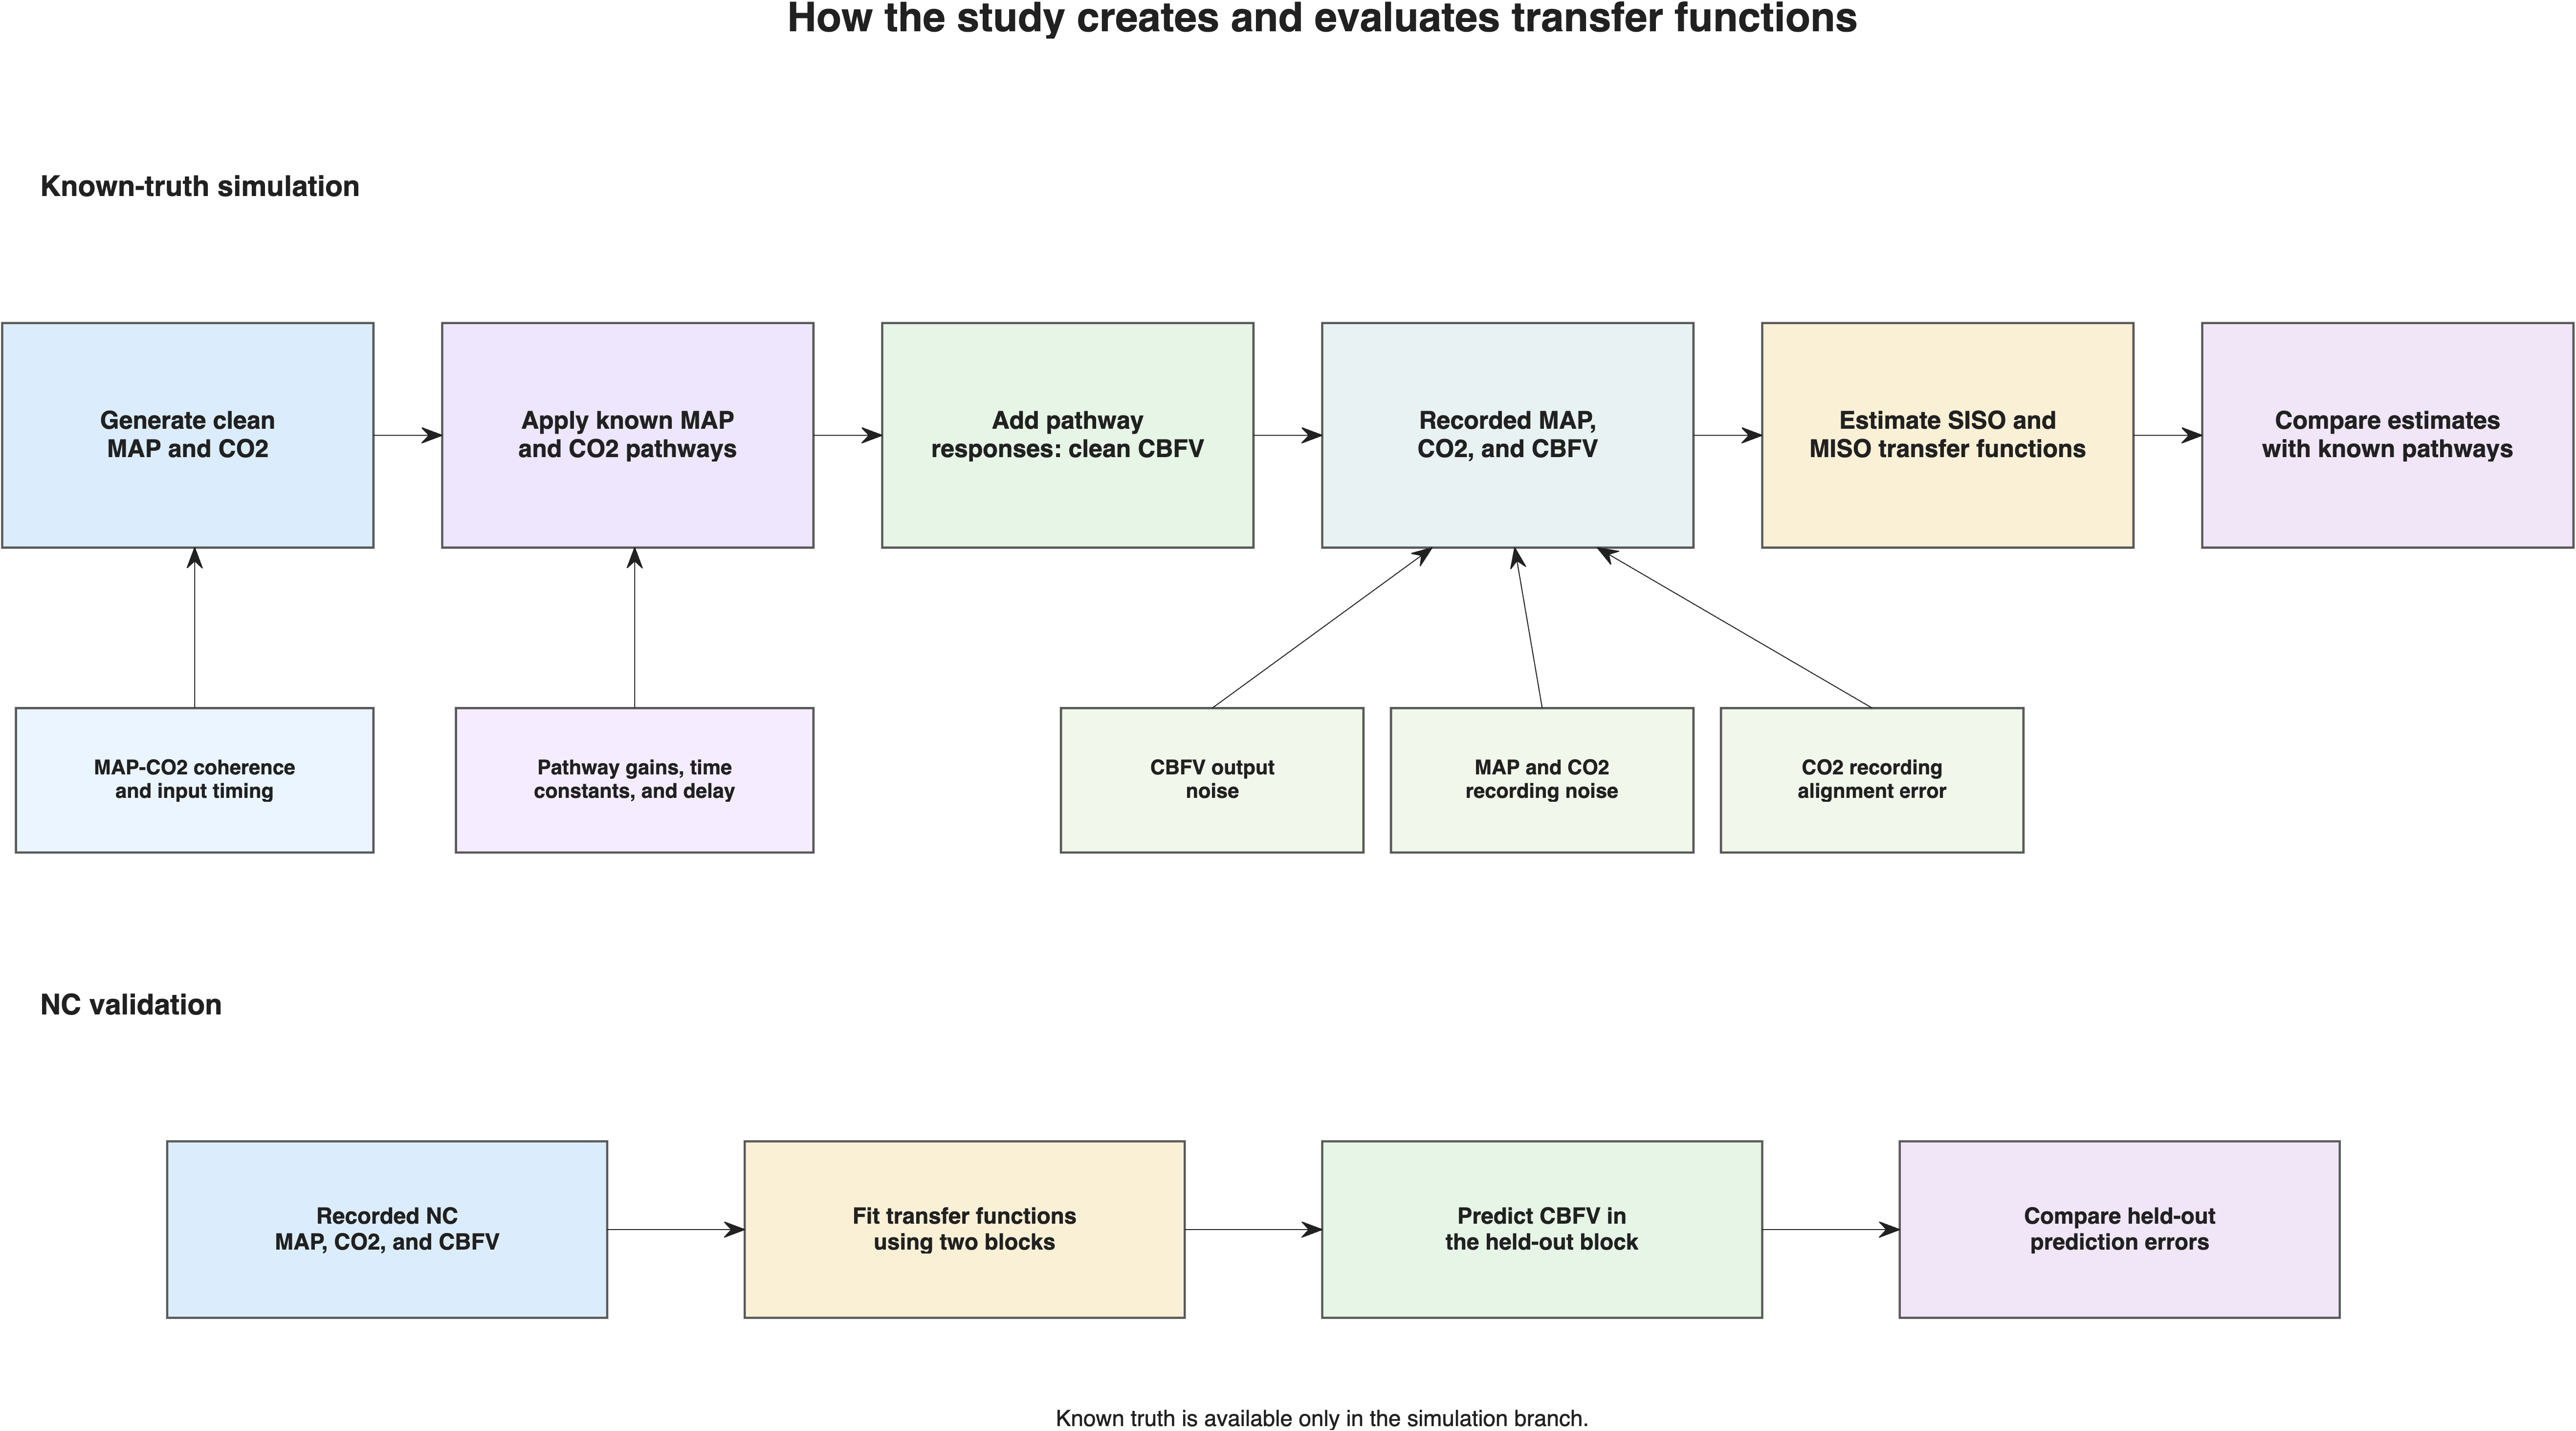
\includegraphics[width=0.94\linewidth]{figure1_study_design.png}
    \caption{Study design. The known-truth branch evaluates recovery of the
    generating MAP and CO$_2$ pathways. The NC branch evaluates held-out block
    prediction with subject-bootstrap uncertainty. Both branches use the same
    spectral estimators but have different accuracy targets.}
    \label{fig:design}
\end{figure}

\section{Methods}

\subsection{Study design and two accuracy questions}

The study contains a known-truth simulation and a held-out analysis of normal
control (NC) recordings (Figure~\ref{fig:design}). The simulation asks whether
SISO or MISO more accurately recovers a transfer function that is known because
it was used to generate the data. The NC analysis asks whether transfer
functions estimated from part of a recording predict CBFV in a different part
of that recording. Human pathway truth is unavailable, so the NC analysis does
not determine which estimated pathway is physiologically correct.

For the simulation, the frequency-specific error for estimator $j$ is

\begin{equation}
E_{j,r}(f) =
\frac{\left|\widehat H_{j,r}(f)-H_r(f)\right|^2}
{\operatorname{mean}_{f\in B}\left|H_r(f)\right|^2},
\label{eq:truth_error}
\end{equation}

where $r$ identifies one simulation replicate, $H_r$ is the known generating
transfer function, $\widehat H_{j,r}$ is its estimate, and $B$ is the
0.02--0.35~Hz reporting band. Because transfer functions contain both a
response magnitude and a timing angle, this complex-valued comparison penalizes
errors in either component. A pathway with zero assigned gain has no meaningful
relative denominator and is evaluated with absolute squared error.

The primary score compares the mean errors from the paired SISO and MISO
analyses:

\begin{equation}
    A(f) = \log_{10}\left(
    \frac{\operatorname{mean}_{r}\{E_{\SISO,r}(f)\}}
    {\operatorname{mean}_{r}\{E_{\MISO,r}(f)\}}
    \right).
    \label{eq:advantage}
\end{equation}

Positive values indicate lower mean error for MISO, negative values indicate
lower mean error for SISO, and zero indicates equal mean error. An advantage of
1 means that mean SISO error is ten times mean MISO error; an advantage of
$-1$ means the reverse. The logarithm places equal error ratios at equal
distances on opposite sides of zero.

\subsection{Frequency, power, and signal-to-noise ratio}

Power describes the average size of a signal's fluctuation around its mean. For
a signal $x$ with $N$ samples, it can be written as

\begin{equation}
P_x=\frac{1}{N}\sum_{n=1}^{N}\left(x_n-\overline{x}\right)^2.
\label{eq:power}
\end{equation}

The power spectrum distributes this total variation across frequency. A larger
power-spectral value means that more of the signal's variation occurs near that
frequency. Signal-to-noise ratio (SNR) compares signal power with added noise
power. At 10~dB, signal power is ten times noise power. At 0~dB, the two powers
are equal. ``No noise'' means that no artificial recording noise was added.

Signals were sampled at 4~Hz, which permits frequencies up to the 2~Hz Nyquist
frequency. Only 0.02--0.35~Hz was reported because this was the prespecified
range of interest. A frequency of 0.10~Hz corresponds to a fluctuation that
repeats approximately every 10 seconds; 0.30~Hz corresponds to approximately
every 3.3 seconds. Spectra were estimated from 100-second, 400-sample Hann
windows with 50\% overlap, linear detrending, and three-bin smoothing. The
resulting simulation-bin spacing was 0.01~Hz. These analysis settings were
identical for SISO and MISO.

\subsection{Known-truth signal generation}

The simulator first generated clean MAP and CO$_2$ signals. It then passed MAP
through a known MAP-to-CBFV transfer function and CO$_2$ through a separate
known CO$_2$-to-CBFV transfer function. The two resulting CBFV contributions
were added to obtain clean CBFV:

\begin{equation}
    Y(f) = H_M(f)M(f) + H_C(f)C(f) + E(f),
    \label{eq:generator}
\end{equation}

where $M$ and $C$ are the generated inputs, $H_M$ and $H_C$ are the known
pathways, and $E$ is added CBFV variation not produced by either pathway. The
MAP pathway used a high-pass-like response with a 3-second time constant. The
CO$_2$ pathway used a low-pass response with a 5-second time constant and a
3-second delay. The assigned CO$_2$-to-MAP gain ratio was defined over the
0.02--0.35~Hz reporting band.

Recording effects were applied after creation of the clean signals. MAP and
CO$_2$ recording noise altered their respective observed input channels. CBFV
output noise altered the observed CBFV channel. The alignment experiment shifted
the recorded CO$_2$ channel relative to MAP and CBFV. These effects are distinct
from the fixed 3-second delay inside the true CO$_2$ pathway. SISO and MISO
always received the same observed signals for a paired comparison.

The transfer function $H_M(f)$ is the CBFV response associated with MAP after
the CO$_2$ contribution is accounted for; $H_C(f)$ is the corresponding CO$_2$
response after accounting for MAP. Transfer-function gain describes response
size, and phase describes response timing relative to the input. The simulator
saved both generating transfer functions before recording noise or alignment
error was applied.

\subsection{NC-derived input-spectrum shape}

Power spectra from the \NCSubjectCount{} NC recordings were used to choose a
plausible frequency distribution for the simulated inputs. MAP and CO$_2$
spectra were calculated using 90-second windows. At each frequency, the median
power across subjects was calculated separately for MAP and CO$_2$. The two
median curves were averaged in decibels and fit from 0.033 to 0.35~Hz to

\begin{equation}
    S_{\mathrm{input}}(f) =
    \frac{1}{1 + (f/f_0)^{\alpha}}.
    \label{eq:input_spectrum}
\end{equation}

The fitted roll-off frequency was $f_0=0.0290$~Hz, the exponent was
$\alpha=2.5514$, and the root-mean-square fitting error was 0.91~dB. Only the
shape was used in the simulator; the measured signal amplitudes and units were
not transferred. MAP and CO$_2$ were assigned the same spectral shape so that
their coherence could be changed without simultaneously changing their
frequency distributions (Figure~\ref{fig:inputspectrum}).

\begin{figure}[H]
    \centering
    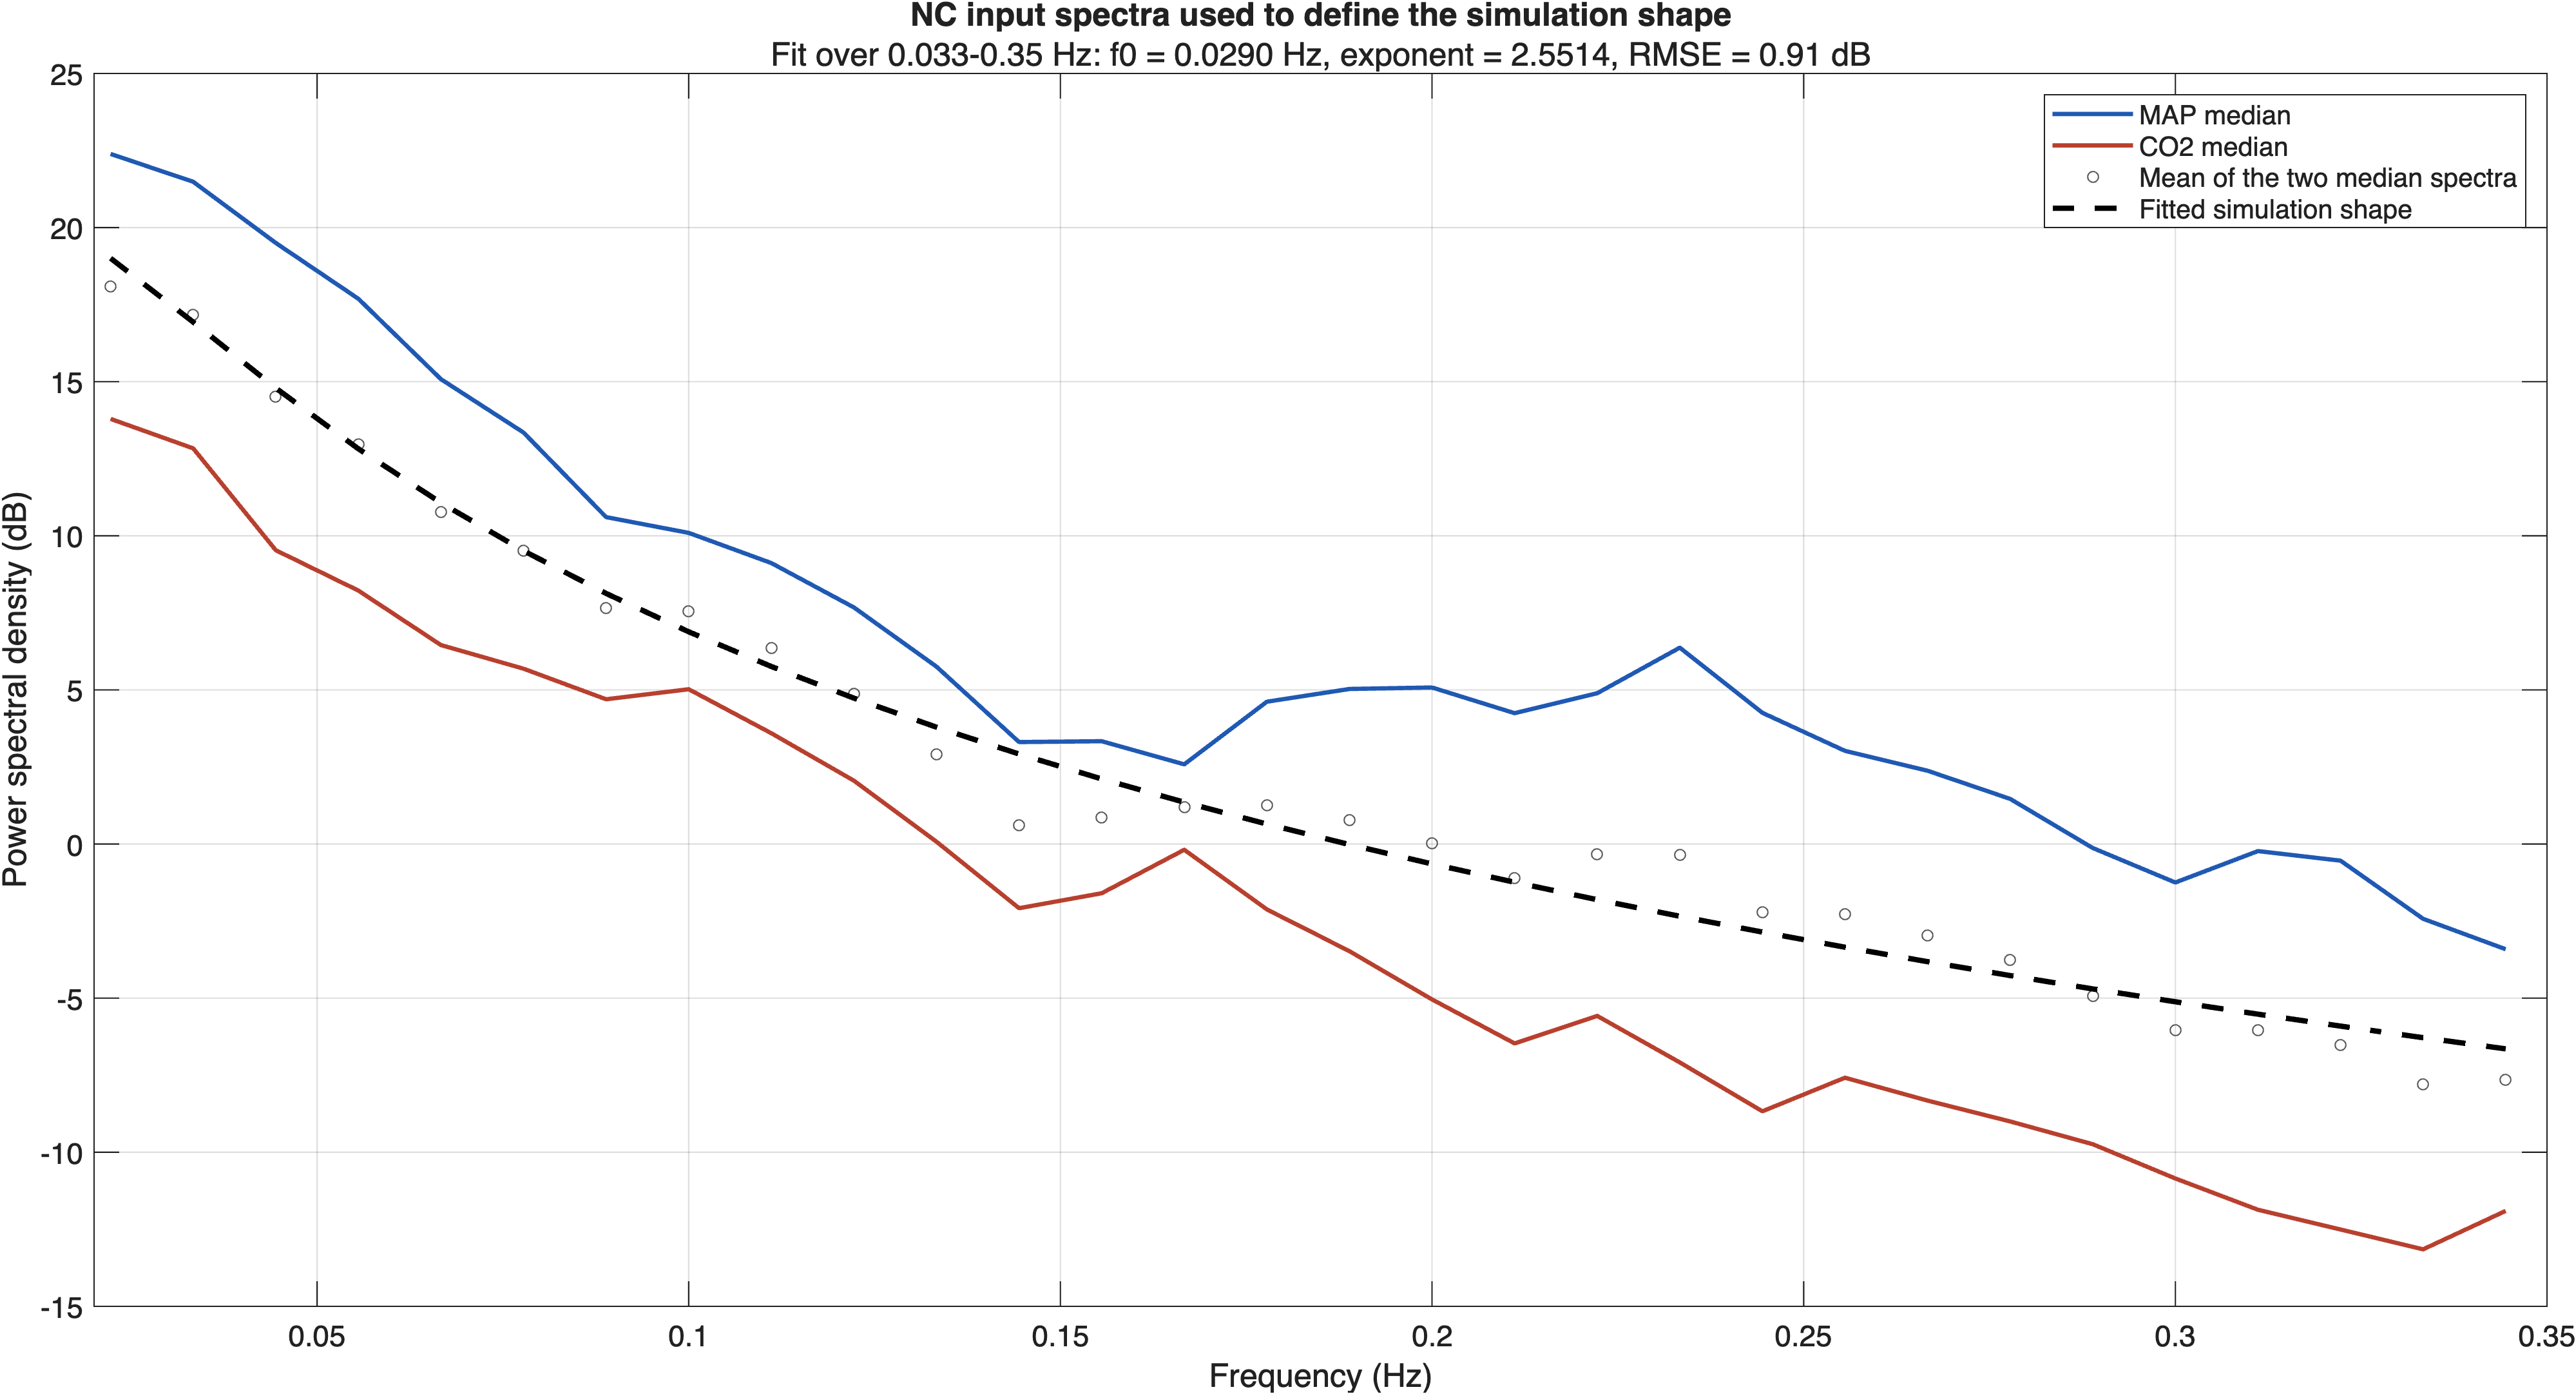
\includegraphics[width=0.92\linewidth]{figure3_nc_input_spectrum.png}
    \caption{Origin of the simulated input-spectrum shape. Curves show the
    subject-median NC MAP and CO$_2$ power spectra, their mean in decibels, and
    the fitted monotonic shape. The fit controls relative power across
    frequency and is not presented as a universal physiological range.}
    \label{fig:inputspectrum}
\end{figure}

\subsection{Tested quantities and fixed reference condition}

MAP--CO$_2$ coherence describes how consistently the two inputs share linear
frequency-specific variation. The NC subject-level bias-corrected band means
had approximate 10th, 50th, and 90th percentiles of 0.065, 0.129, and 0.177.
We therefore included 0.15 as the NC-informed operating level, 0 as an
independent-input control, and 0.50 and 0.95 as increasingly strong dependence
tests.

The displayed heatmaps vary one quantity at a time. Except for the named
quantity, the primary maps use 300 seconds of data, 10~dB signal-shaped CBFV
output noise, MAP--CO$_2$ coherence 0.50, and an assigned CO$_2$-to-MAP pathway
gain ratio of 1. Coherence 0.50 is a moderate-dependence test condition rather
than an NC-derived default. Likewise, pathway ratio 1 and output SNR 10~dB are
declared mechanism and recording-quality conditions; they were not estimated
from the NC recordings.

The primary maps vary input coherence, relative CO$_2$ pathway strength,
recording duration, and CBFV output SNR. Separate sensitivity analyses vary
MAP input noise, CO$_2$ input noise, MAP--CO$_2$ input lag, and CO$_2$
recording alignment. MAP and CO$_2$ input noise were changed separately, with
the other input kept noise-free. The primary CBFV noise had the same spectral
shape as clean CBFV but an independent random phase. A white-noise check tested
whether conclusions depended on that frequency shape. Table~\ref{tab:design}
lists every tested level and the values held fixed.

\begin{table}[H]
    \centering
    \caption{Simulation quantities, tested levels, fixed settings, and the
    basis for selecting each level.}
    \label{tab:design}
    \scriptsize
    \begin{tabularx}{\linewidth}{@{}p{0.17\linewidth}p{0.17\linewidth}p{0.29\linewidth}X@{}}
\toprule
Varied quantity & Tested levels & Other settings held fixed & Basis for levels \\
\midrule
MAP--CO$_2$ coherence & 0, 0.15, 0.50, 0.95 & 300 s; 10 dB CBFV SNR; pathway ratio 1 & 0.15 is NC-informed; 0 is a control; 0.50 and 0.95 are stress levels \\
Relative CO$_2$ pathway strength & 0, 0.25, 1 & 300 s; 10 dB CBFV SNR; coherence 0.50 & Mechanistic absent, weaker, and equal-gain conditions \\
Recording duration & 300, 600 s & 10 dB CBFV SNR; coherence 0.50; pathway ratio 1 & 300 s reflects the NC recording length; 600 s tests more data \\
CBFV output SNR & no noise, 10, 0 dB & 300 s; coherence 0.50; pathway ratio 1 & Chosen clean, moderate, and severe noise conditions \\
MAP--CO$_2$ input lag & -6, 0, 4 s & 300 s; 10 dB CBFV SNR; pathway ratio 1; coherence shown separately & Approximate NC lag quantiles, used as sensitivity levels \\
MAP input SNR & no noise, 10, 0 dB & CO$_2$ input clean; 300 s; 10 dB CBFV SNR; coherence 0.50; ratio 1 & Chosen recording-quality levels \\
CO$_2$ input SNR & no noise, 10, 0 dB & MAP input clean; same reference settings & Chosen recording-quality levels \\
CO$_2$ alignment error & -3, 0, 3 s & Both inputs clean; same reference settings & Acquisition robustness check \\
\bottomrule
\end{tabularx}

\end{table}

The input-lag analysis changes the timing relationship between generated MAP
and CO$_2$. Its levels of $-6$, 0, and 4 seconds approximate the 10th, median,
and 90th percentiles from the NC phase-lag fits. It does not independently set
MAP-to-CBFV or CO$_2$-to-CBFV phase. Those phases follow from the fixed pathway
responses and are measured as outcomes.

\subsection{SISO and MISO estimation}

At each frequency, $S_{MM}$ and $S_{CC}$ denote MAP and CO$_2$ power.
$S_{MC}$ and $S_{CM}$ describe their shared variation, while $S_{MY}$ and
$S_{CY}$ describe how each input varies with CBFV. These are frequency-specific
counterparts of variance and covariance.

MISO estimates the two pathways simultaneously:

\begin{equation}
\begin{bmatrix} \widehat H_M \\ \widehat H_C \end{bmatrix}
=
\begin{bmatrix} S_{MM} & S_{MC} \\ S_{CM} & S_{CC} \end{bmatrix}^{-1}
\begin{bmatrix} S_{MY} \\ S_{CY} \end{bmatrix}.
\label{eq:miso}
\end{equation}

This is equivalent to estimating the MAP response while accounting for CO$_2$
and estimating the CO$_2$ response while accounting for MAP. Each resulting
transfer function has a gain and phase at every frequency.

For comparison, the MAP-only SISO estimate can be written approximately as

\begin{equation}
\widehat H_{M,\SISO}(f)
= H_M(f) + H_C(f)\frac{S_{CM}(f)}{S_{MM}(f)}
  + \frac{S_{EM}(f)}{S_{MM}(f)}.
\label{eq:siso_bias}
\end{equation}

The second term shows how a MAP-only estimate can contain part of the CO$_2$
pathway when MAP and CO$_2$ vary together. The last term represents unexplained
and finite-record error. SISO therefore answers a pairwise MAP--CBFV question,
whereas MISO attempts to separate the conditional MAP and CO$_2$ pathways.
The same reasoning applies to the CO$_2$-only SISO comparison.

\subsection{Simulation replicates and uncertainty}

A condition is one fixed combination of coherence, pathway strength, duration,
noise, and timing settings. The condition was repeated using 500 independent
random signal realizations. We refer to each repetition as a simulation
replicate. Within a replicate, training and validation signals had the same
generating pathways and condition settings but independent random fluctuations.
Every SISO estimate was paired with a MISO estimate obtained from the same
observed signals (Figure~\ref{fig:replicates}).

\begin{figure}[H]
    \centering
    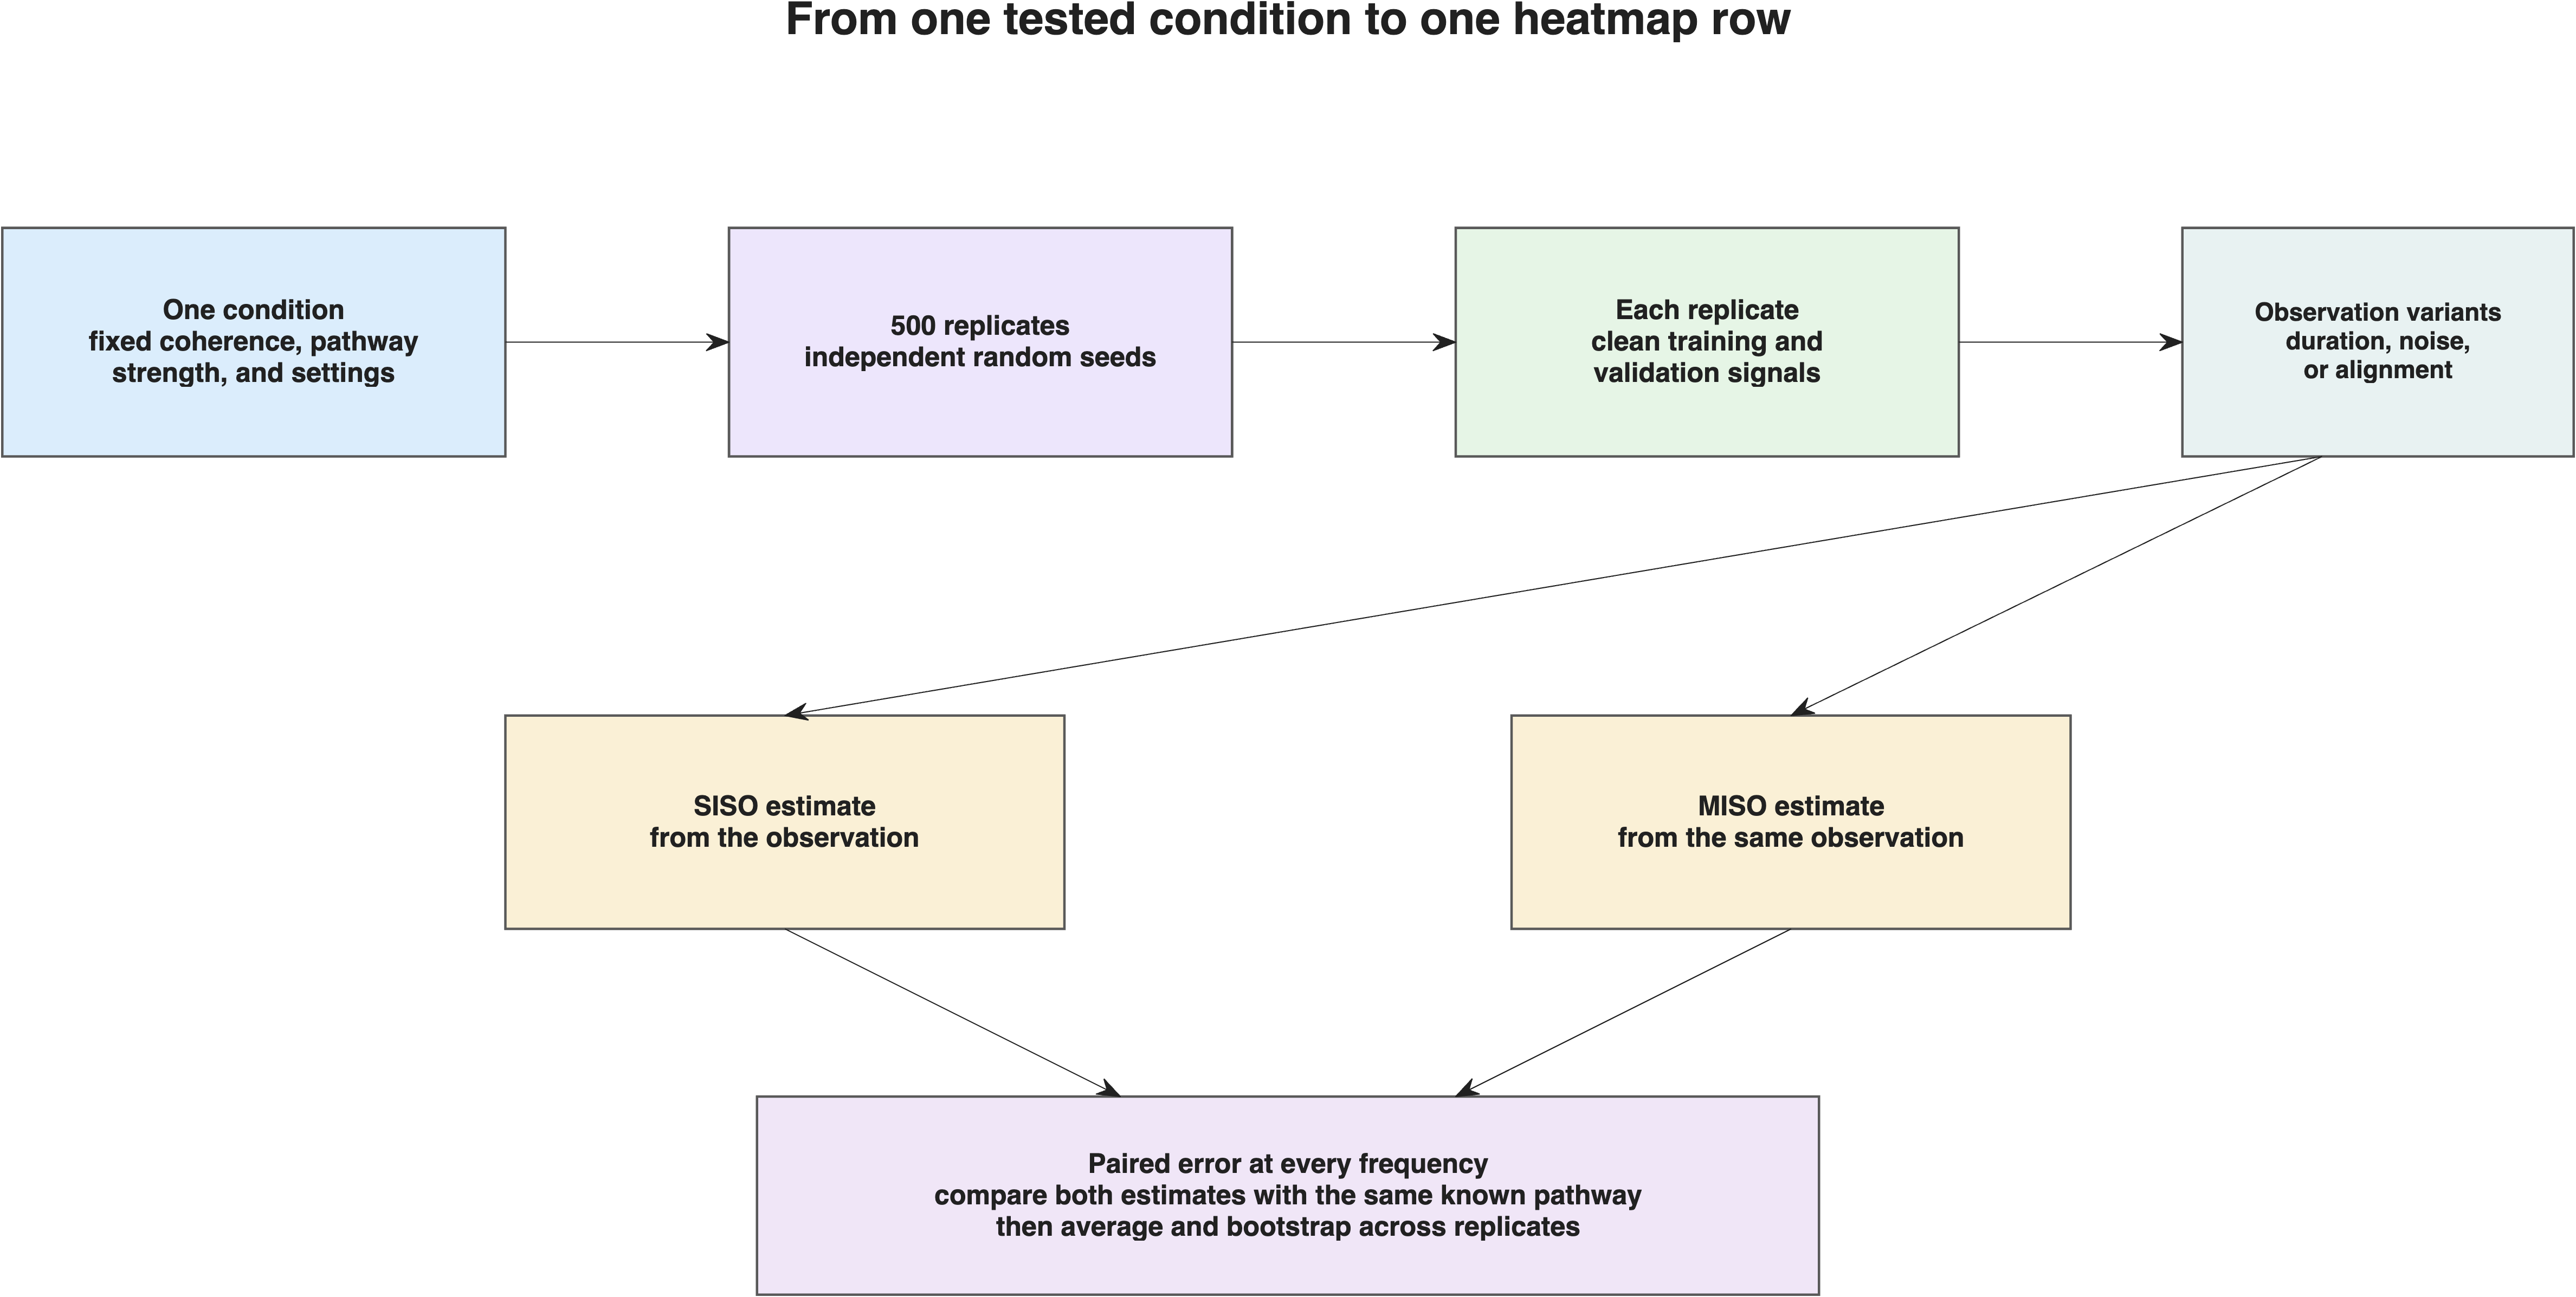
\includegraphics[width=0.95\linewidth]{figure2_simulation_replicates.png}
    \caption{Simulation hierarchy. Each tested condition was repeated with
    500 random signal realizations. Observation variants were derived under the
    declared condition, and SISO and MISO were evaluated on the same data before
    errors were averaged across replicates.}
    \label{fig:replicates}
\end{figure}

The simulation was repeated because a finite random recording can produce a
different estimate each time even when its underlying condition is unchanged.
To measure the remaining numerical uncertainty, the 500 paired replicate
errors were resampled together 2,000 times. The standard deviation of these
resampled advantages is the Monte Carlo standard error. The prespecified target
was a maximum standard error of 0.05 advantage units in every finite primary
heatmap cell. Table~\ref{tab:precision} reports whether that target was met.

\begin{table}[H]
    \centering
    \caption{Numerical precision of the four primary heatmaps.}
    \label{tab:precision}
    \small
    \begin{tabular}{lrrrr}
\toprule
Map & Maximum MC SE & Finite cells & Passing cells & Paired N \\
\midrule
input coherence & 0.0310 & 136 & 136 & 500--500 \\
co2 pathway ratio & 0.0276 & 102 & 102 & 500--500 \\
recording duration & 0.0276 & 68 & 68 & 500--500 \\
output snr & 0.0276 & 102 & 102 & 500--500 \\
\bottomrule
\end{tabular}

\end{table}

As an implementation check, the expected population SISO mixing error was also
calculated directly from the known input spectra and pathways. Agreement between
that expected error and the long-record empirical SISO result verifies that the
observed SISO error arises from the omitted input as intended. This quantity was
used to check the simulator and was not treated as another study endpoint.

\subsection{Held-out NC validation}

Each NC recording was divided into three non-overlapping 90-second blocks.
Transfer functions were estimated from two blocks and evaluated by their CBFV
prediction error in the third. Each block served once as the held-out block.
Fold errors were averaged within each of the \NCSubjectCount{} subjects, after
which subjects were resampled 2,000 times to obtain pointwise 95\% bootstrap
intervals. The NC SISO comparator used MAP alone; MISO used MAP and CO$_2$.
This analysis measures held-out prediction and does not compare either model
with an unknown human transfer-function truth.

\subsection{Reproducibility}

Random seeds, simulation settings, exact factor selections, source tables, and
the MATLAB version were saved with the final study. Manuscript figures are
regenerated from those saved outputs without rerunning or altering the study.
Running \texttt{buildManuscript} recreates the figures, tables, and canonical
PDF from the archived numerical results.

\section{Results}

The simulation results use the same layout throughout. Frequency is on the
horizontal axis, the tested level of one quantity is on the vertical axis, and
color shows the MISO advantage. Positive values indicate lower recovery error
with MISO; negative values indicate lower recovery error with SISO. In every
panel, only the named quantity changes. The other quantities remain at the
values stated in the caption and Table~\ref{tab:design}.

\subsection{Production completion and precision}

The final production archive contained \SimulationTotalAnalyses{} paired
analyses across the primary and sensitivity experiments. All finite cells in
the four primary heatmaps met the prespecified Monte Carlo standard-error
target of 0.05 advantage units. The largest observed standard error was
\MaximumMonteCarloSE{}, with 500 paired replicates in each finite cell
(Table~\ref{tab:precision}). Thus, repeating the same conditions with additional
random signals would be unlikely to materially change the broad heatmap
patterns.

\subsection{Primary MAP-pathway recovery}

Figure~\ref{fig:mapprimary} shows the frequency-by-factor MAP-pathway
advantage maps. The color scale is centered at zero so that positive regions
indicate lower MAP-pathway error for MISO and negative regions indicate lower
error for SISO. The pattern is frequency-specific rather than a single global
ranking of the two estimators.

The input-coherence panel shows positive MISO advantage across the retained
frequencies at coherence 0, 0.15, and 0.50. At coherence 0.95, the mean
advantage was close to zero and the heatmap contained both positive and
negative frequencies. Moderate shared variation allowed the MAP-only SISO
estimate to contain part of the CO$_2$ pathway. At very high coherence, MAP
and CO$_2$ carried less independent information, making it harder for MISO to
separate their contributions.

The pathway-strength panel shows the complementary result. When the CO$_2$
pathway was absent, MAP-only SISO had lower MAP-pathway recovery error. In that
condition there was no second pathway for SISO to omit, while MISO still
estimated an additional coefficient. When the assigned CO$_2$ pathway was as
strong as the MAP pathway, MISO had lower error across the retained band. The
intermediate level produced a transition between those two cases.

Increasing recording duration from 300 to 600 seconds increased the MISO
advantage throughout the reporting band. In contrast, reducing CBFV output SNR
reduced the advantage. With no added output noise or with 10-dB SNR, every
reported frequency favored MISO. At 0-dB SNR, where unexplained and
pathway-driven CBFV had equal power, the average advantage approached zero and
19 of 34 frequencies favored SISO.

\begin{figure}[H]
    \centering
    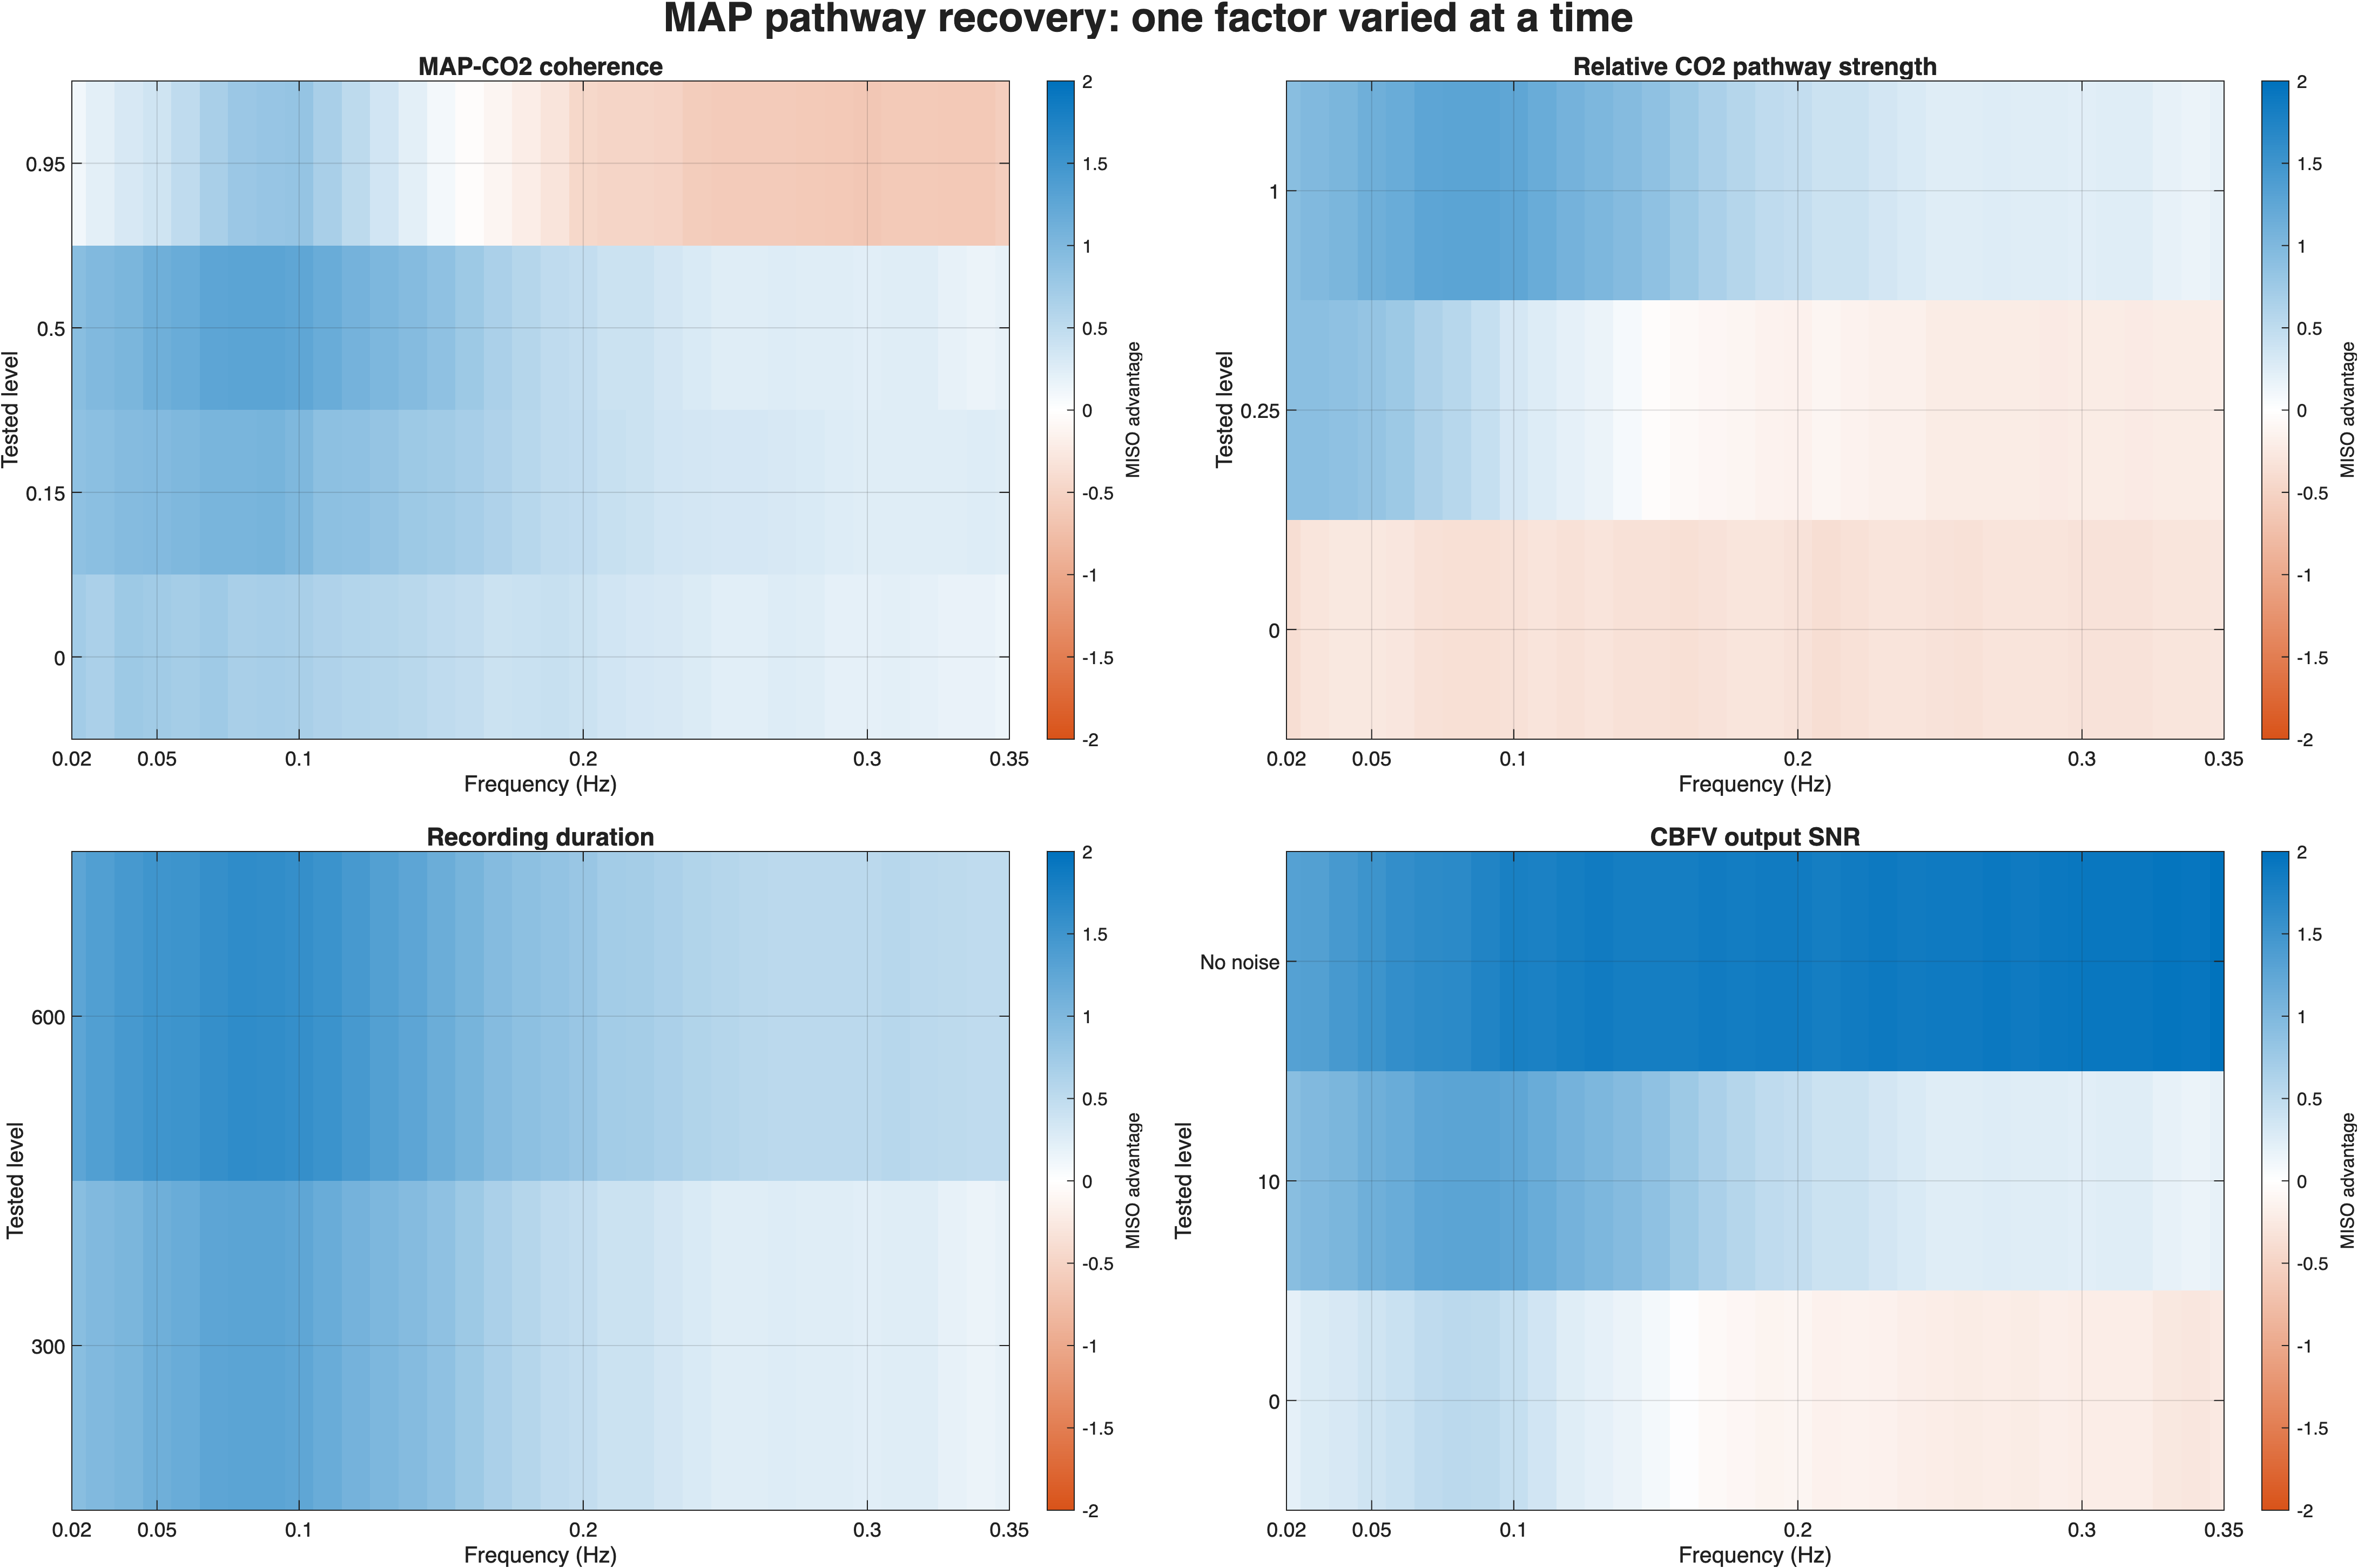
\includegraphics[width=\linewidth]{figure2_map_primary_factors.png}
    \caption{MAP-pathway recovery when one quantity was varied at a time.
    Input coherence was varied with duration 300~s, output SNR 10~dB, and
    CO$_2$-to-MAP pathway ratio 1. Pathway ratio was varied with duration
    300~s, output SNR 10~dB, and coherence 0.50. Duration was varied with
    output SNR 10~dB, coherence 0.50, and pathway ratio 1. Output SNR was
    varied with duration 300~s, coherence 0.50, and pathway ratio 1. Inputs
    were otherwise clean and aligned, with zero MAP--CO$_2$ lag. Positive
    values favor MISO; negative values favor MAP-only SISO.}
    \label{fig:mapprimary}
\end{figure}

\subsection{Primary CO$_2$-pathway recovery}

The CO$_2$-pathway maps are shown separately in
Figure~\ref{fig:co2primary}. These panels compare MISO with CO$_2$-only SISO and
therefore ask whether the CO$_2$ response was recovered more accurately after
accounting for MAP. The same main boundaries were present: MISO benefited from
a meaningful second pathway and longer recordings, whereas very high input
coherence and severe output noise reduced its advantage. The MAP and CO$_2$
results are kept separate because good recovery of one pathway does not imply
good recovery of the other.

\begin{figure}[H]
    \centering
    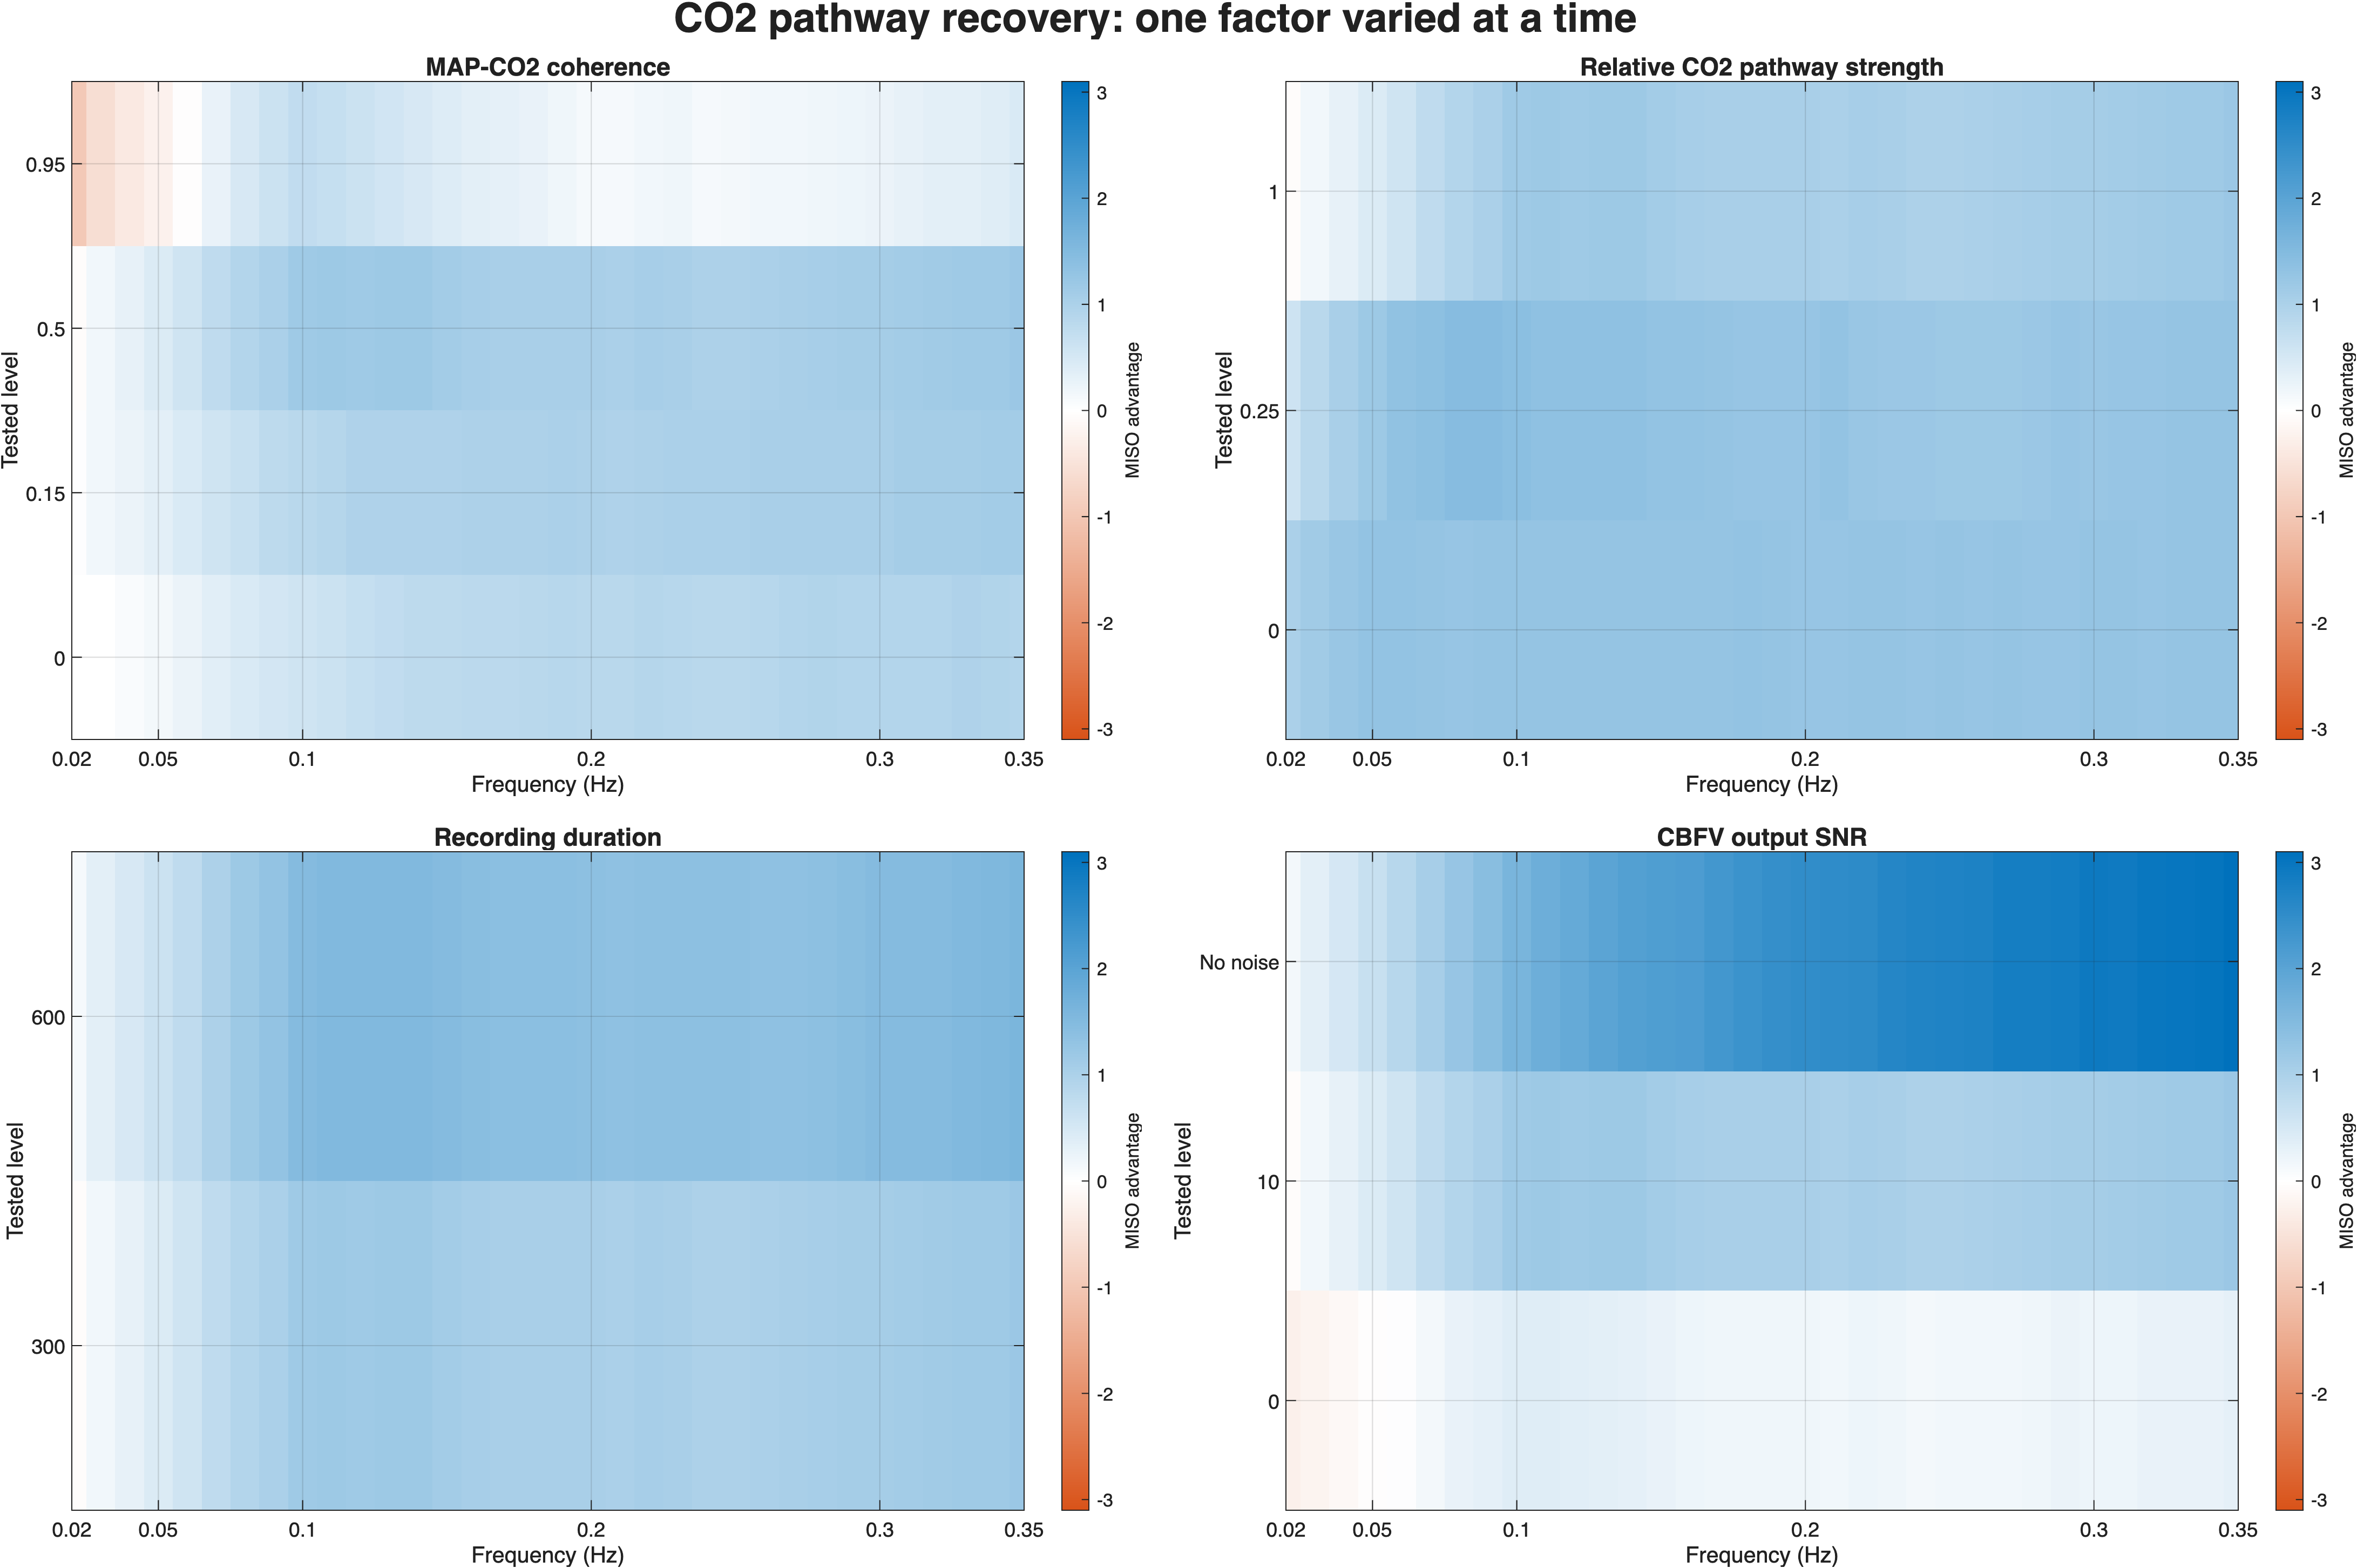
\includegraphics[width=\linewidth]{figure3_co2_primary_factors.png}
    \caption{CO$_2$-pathway recovery when one quantity was varied at a time.
    The fixed settings in the four panels are the same as in
    Figure~\ref{fig:mapprimary}. Positive values favor MISO; negative values
    favor CO$_2$-only SISO.}
    \label{fig:co2primary}
\end{figure}

\subsection{Recording sensitivity}

Figure~\ref{fig:sensitivity} varies MAP recording noise, CO$_2$ recording
noise, and CO$_2$ alignment error separately. Increasing noise in either input
reduced the information available to estimate its pathway. Shifting the
recorded CO$_2$ signal away from the timing used to generate CBFV also weakened
the comparison. These panels describe sensitivity to recording and processing
conditions; they do not represent changes in the underlying pathways.

\begin{figure}[H]
    \centering
    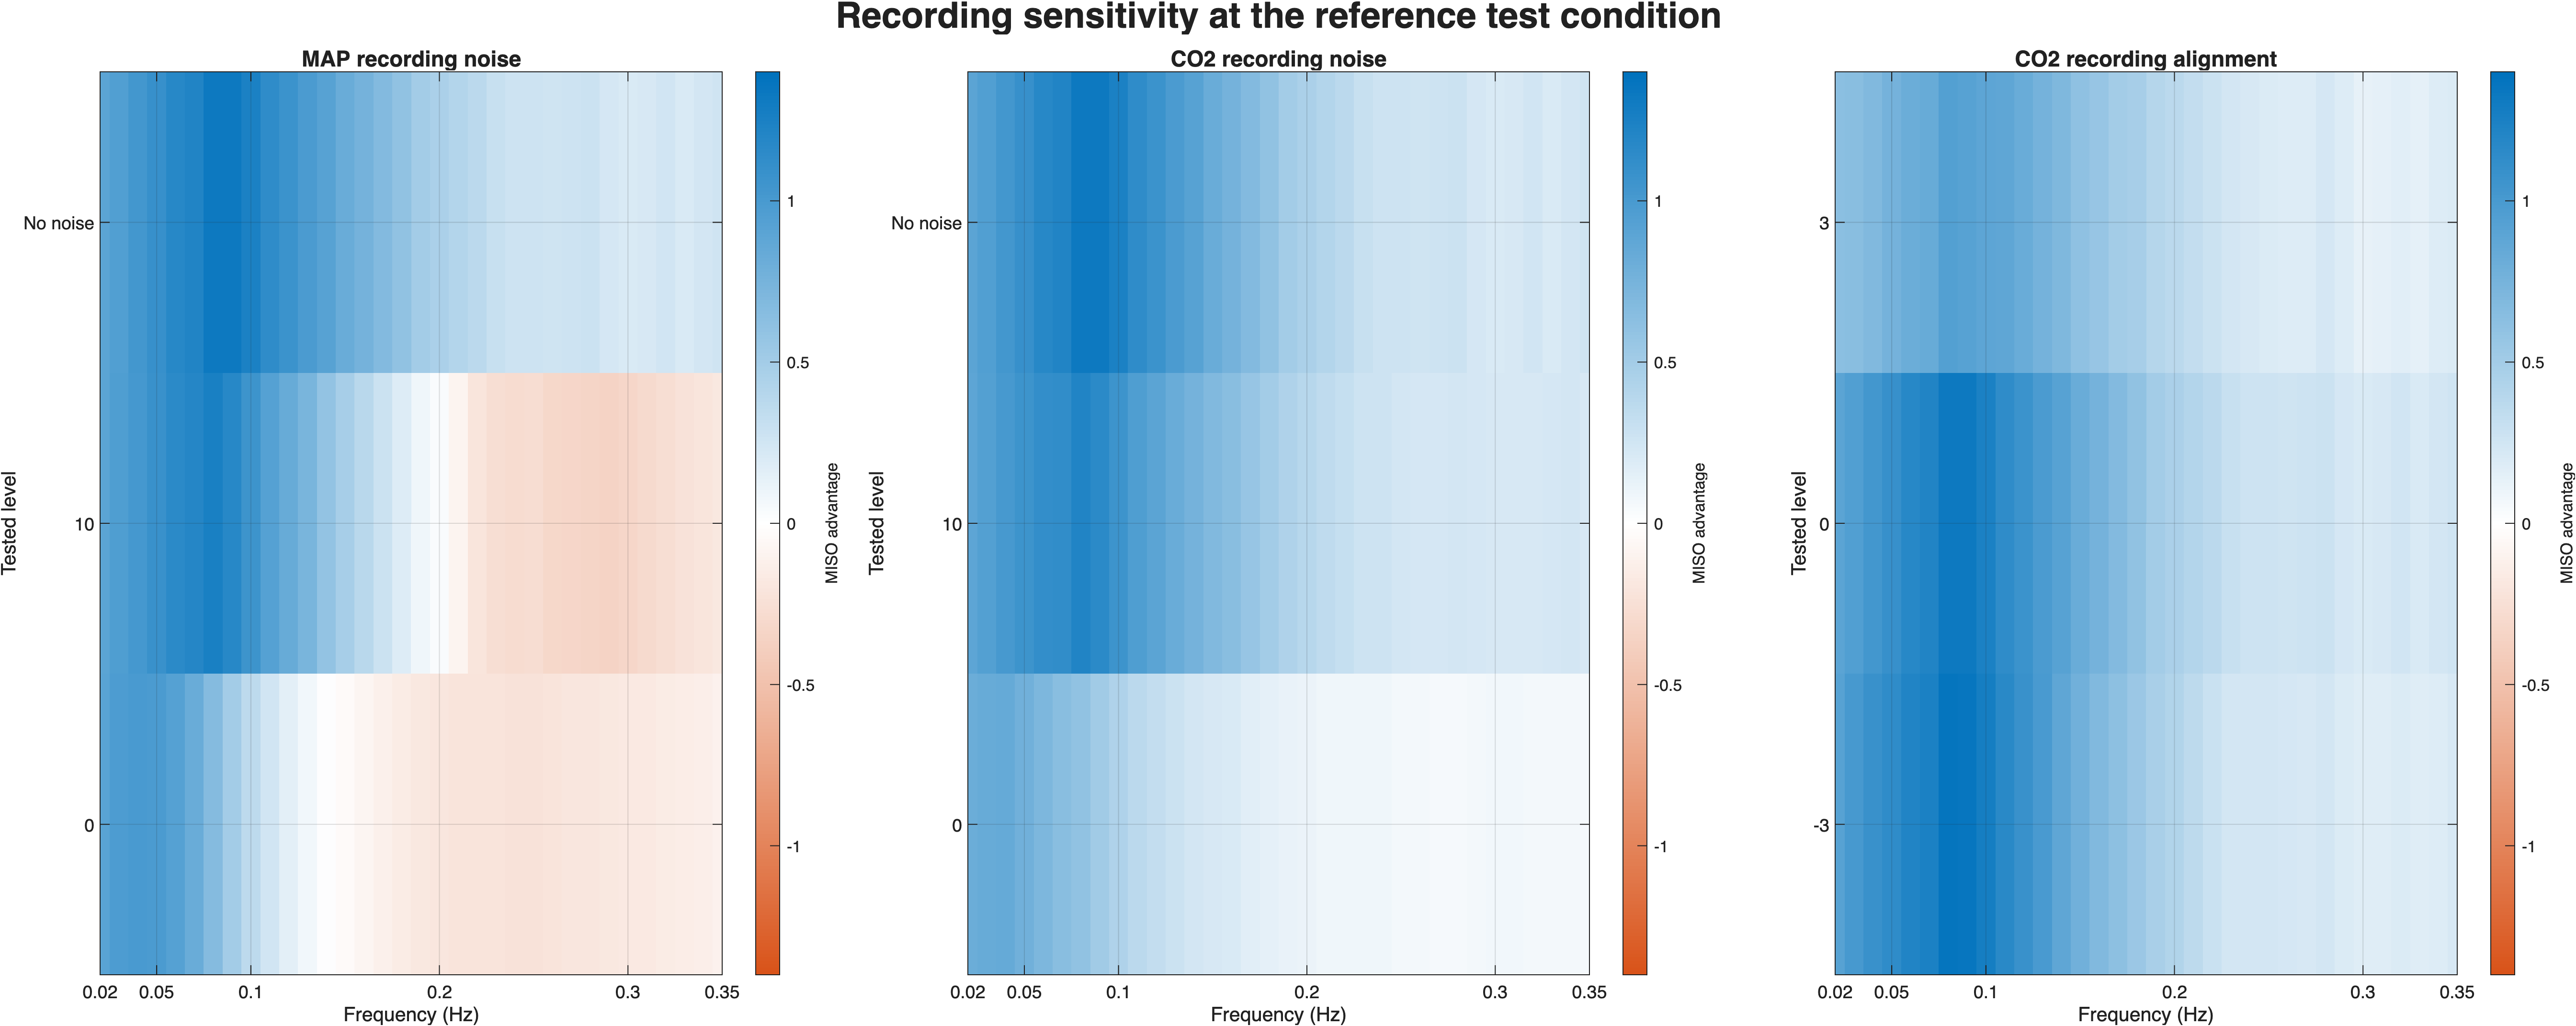
\includegraphics[width=\linewidth]{figure4_phase_and_robustness.png}
    \caption{MAP-pathway sensitivity to input recording quality and alignment.
    Each panel varies only its named quantity. All panels use duration 300~s,
    output SNR 10~dB, input coherence 0.50, pathway ratio 1, and zero
    MAP--CO$_2$ lag. When MAP noise varies, CO$_2$ remains noise-free; when
    CO$_2$ noise varies, MAP remains noise-free. The alignment panel uses
    noise-free inputs. Positive values favor MISO; negative values favor
    MAP-only SISO.}
    \label{fig:sensitivity}
\end{figure}

\subsection{Timing sensitivity}

The MAP--CO$_2$ lag experiment is shown at three input-coherence levels in
Figure~\ref{fig:phaselevels}. At coherence 0.15 and 0.50, MISO advantage
remained positive across the tested timing levels. At coherence 0.95, the maps
contained both positive and negative regions. Thus, the effect of timing
depended on whether the two inputs still contained enough independent
frequency-specific variation to separate their pathways.

\begin{figure}[H]
    \centering
    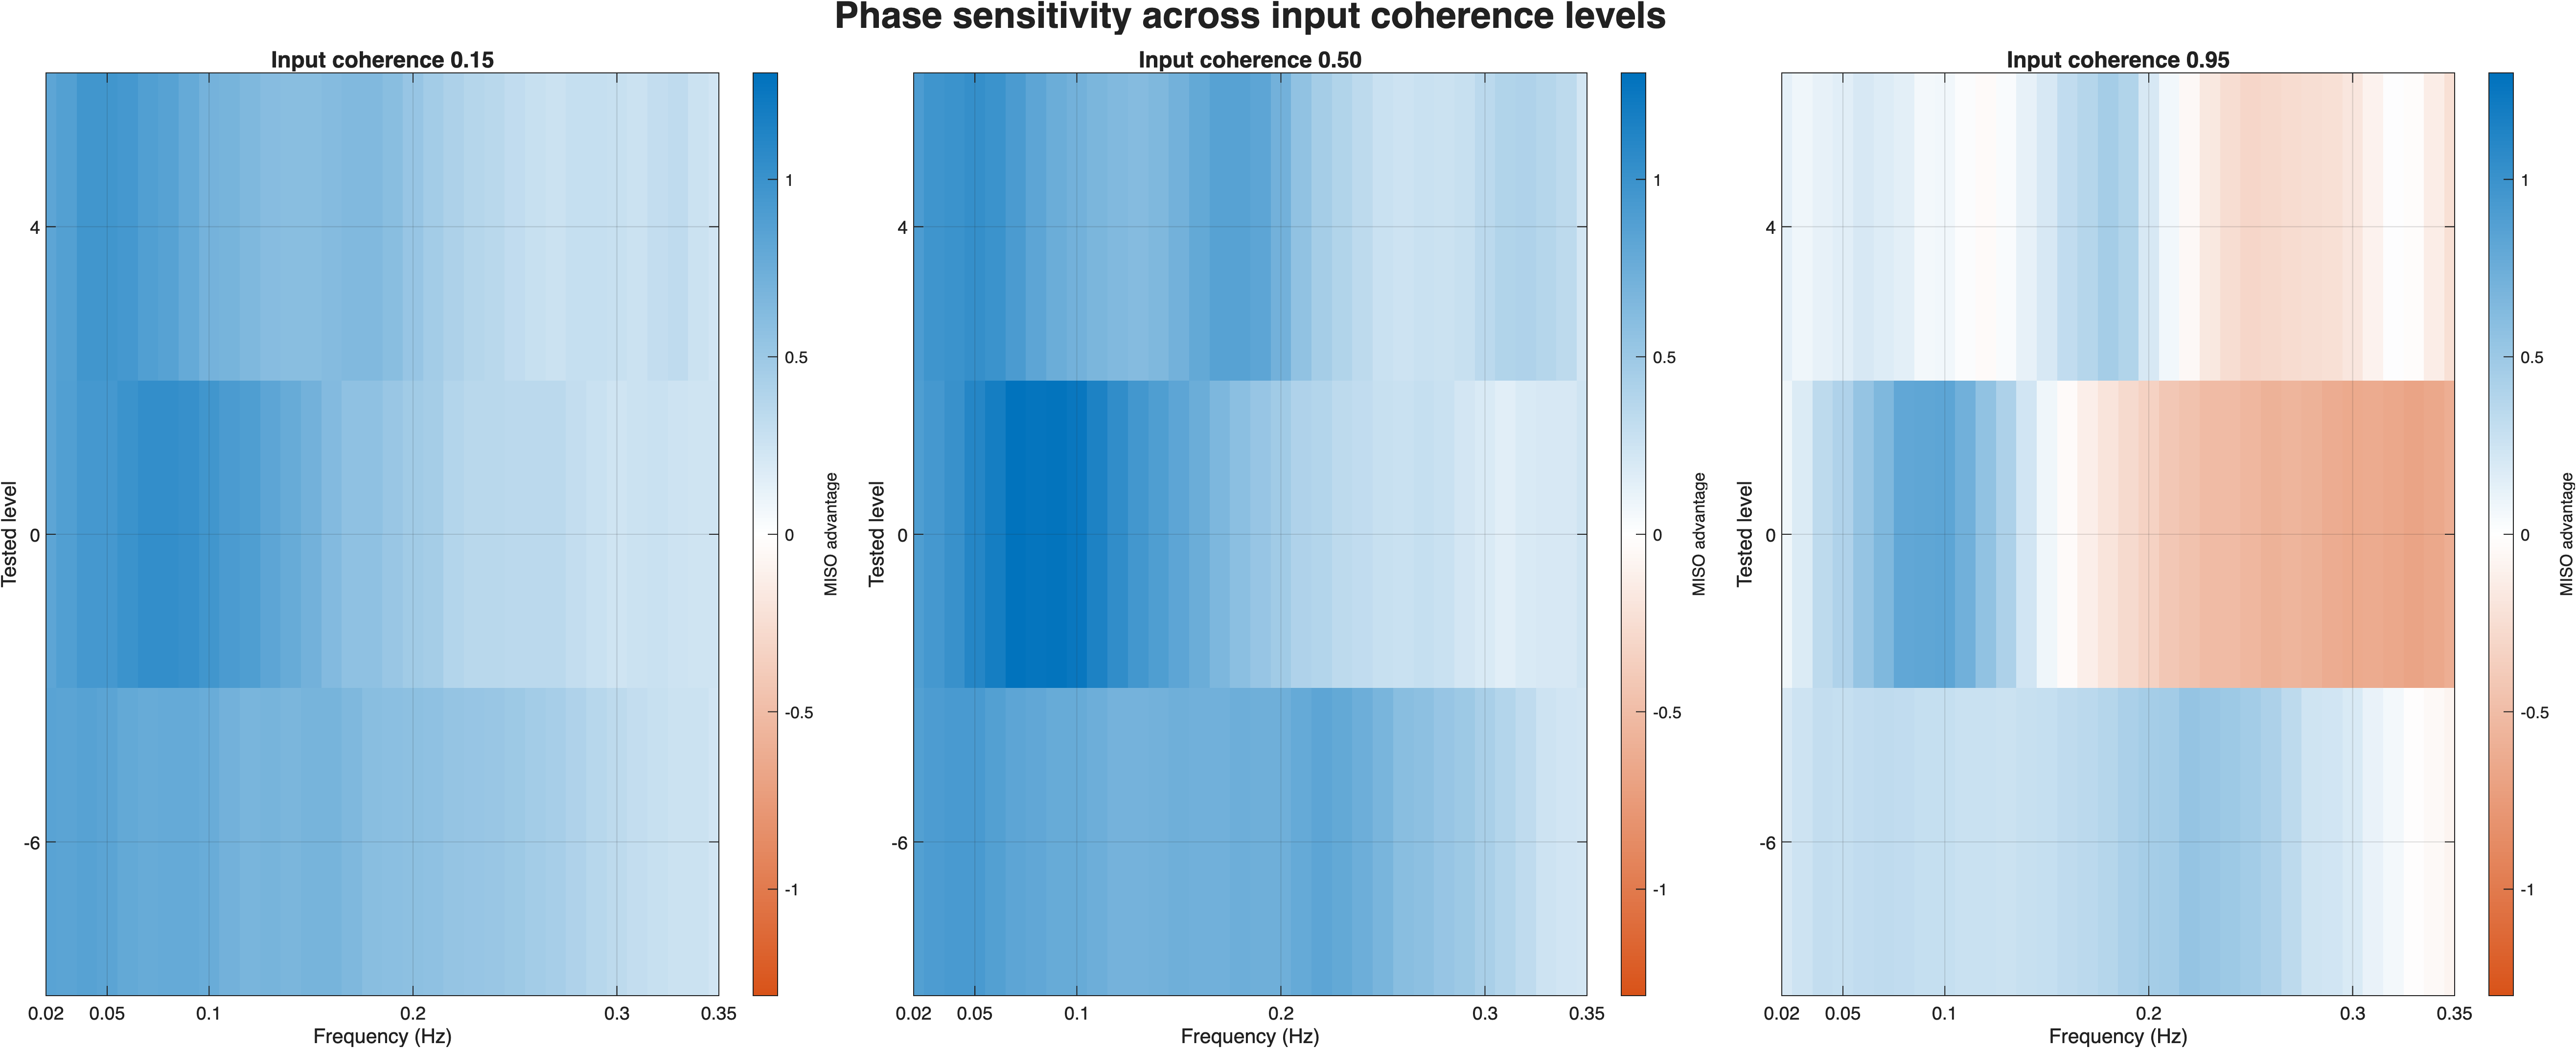
\includegraphics[width=\linewidth]{figure7_phase_levels.png}
    \caption{MAP-pathway sensitivity to MAP--CO$_2$ timing at input coherence
    0.15, 0.50, and 0.95. Within each panel, lag is varied while duration is
    fixed at 300~s, output SNR at 10~dB, pathway ratio at 1, and inputs are
    noise-free and aligned. Positive values favor MISO; negative values favor
    MAP-only SISO.}
    \label{fig:phaselevels}
\end{figure}

\subsection{Held-out NC validation}

The NC analysis used prediction of held-out CBFV because the true human
transfer functions were unknown. Across all \NCFrequencyCount{} retained
frequencies, MISO advantage ranged from \NCAdvantageMinimum{} to
\NCAdvantageMaximum{} and all \NCNegativeCount{} point estimates were negative
(Figure~\ref{fig:nc}). The 95\% pointwise bootstrap interval was entirely below
zero at \NCBelowZeroCount{} frequencies and included zero at
\NCIncludesZeroCount{} frequencies. Under this protocol, MAP-only SISO
predicted the held-out NC blocks more accurately than MISO over the analyzed
band.

This result does not contradict a positive MISO truth-recovery advantage in
some simulation conditions. The endpoints differ. The simulation measures
recovery of known MAP and CO$_2$ pathways, whereas the NC analysis measures
prediction of CBFV without access to the true human pathways. The NC result
therefore supports MAP-only SISO for this held-out prediction task and dataset;
it does not establish which estimator recovered the unknown physiological
pathways more accurately.

\begin{figure}[H]
    \centering
    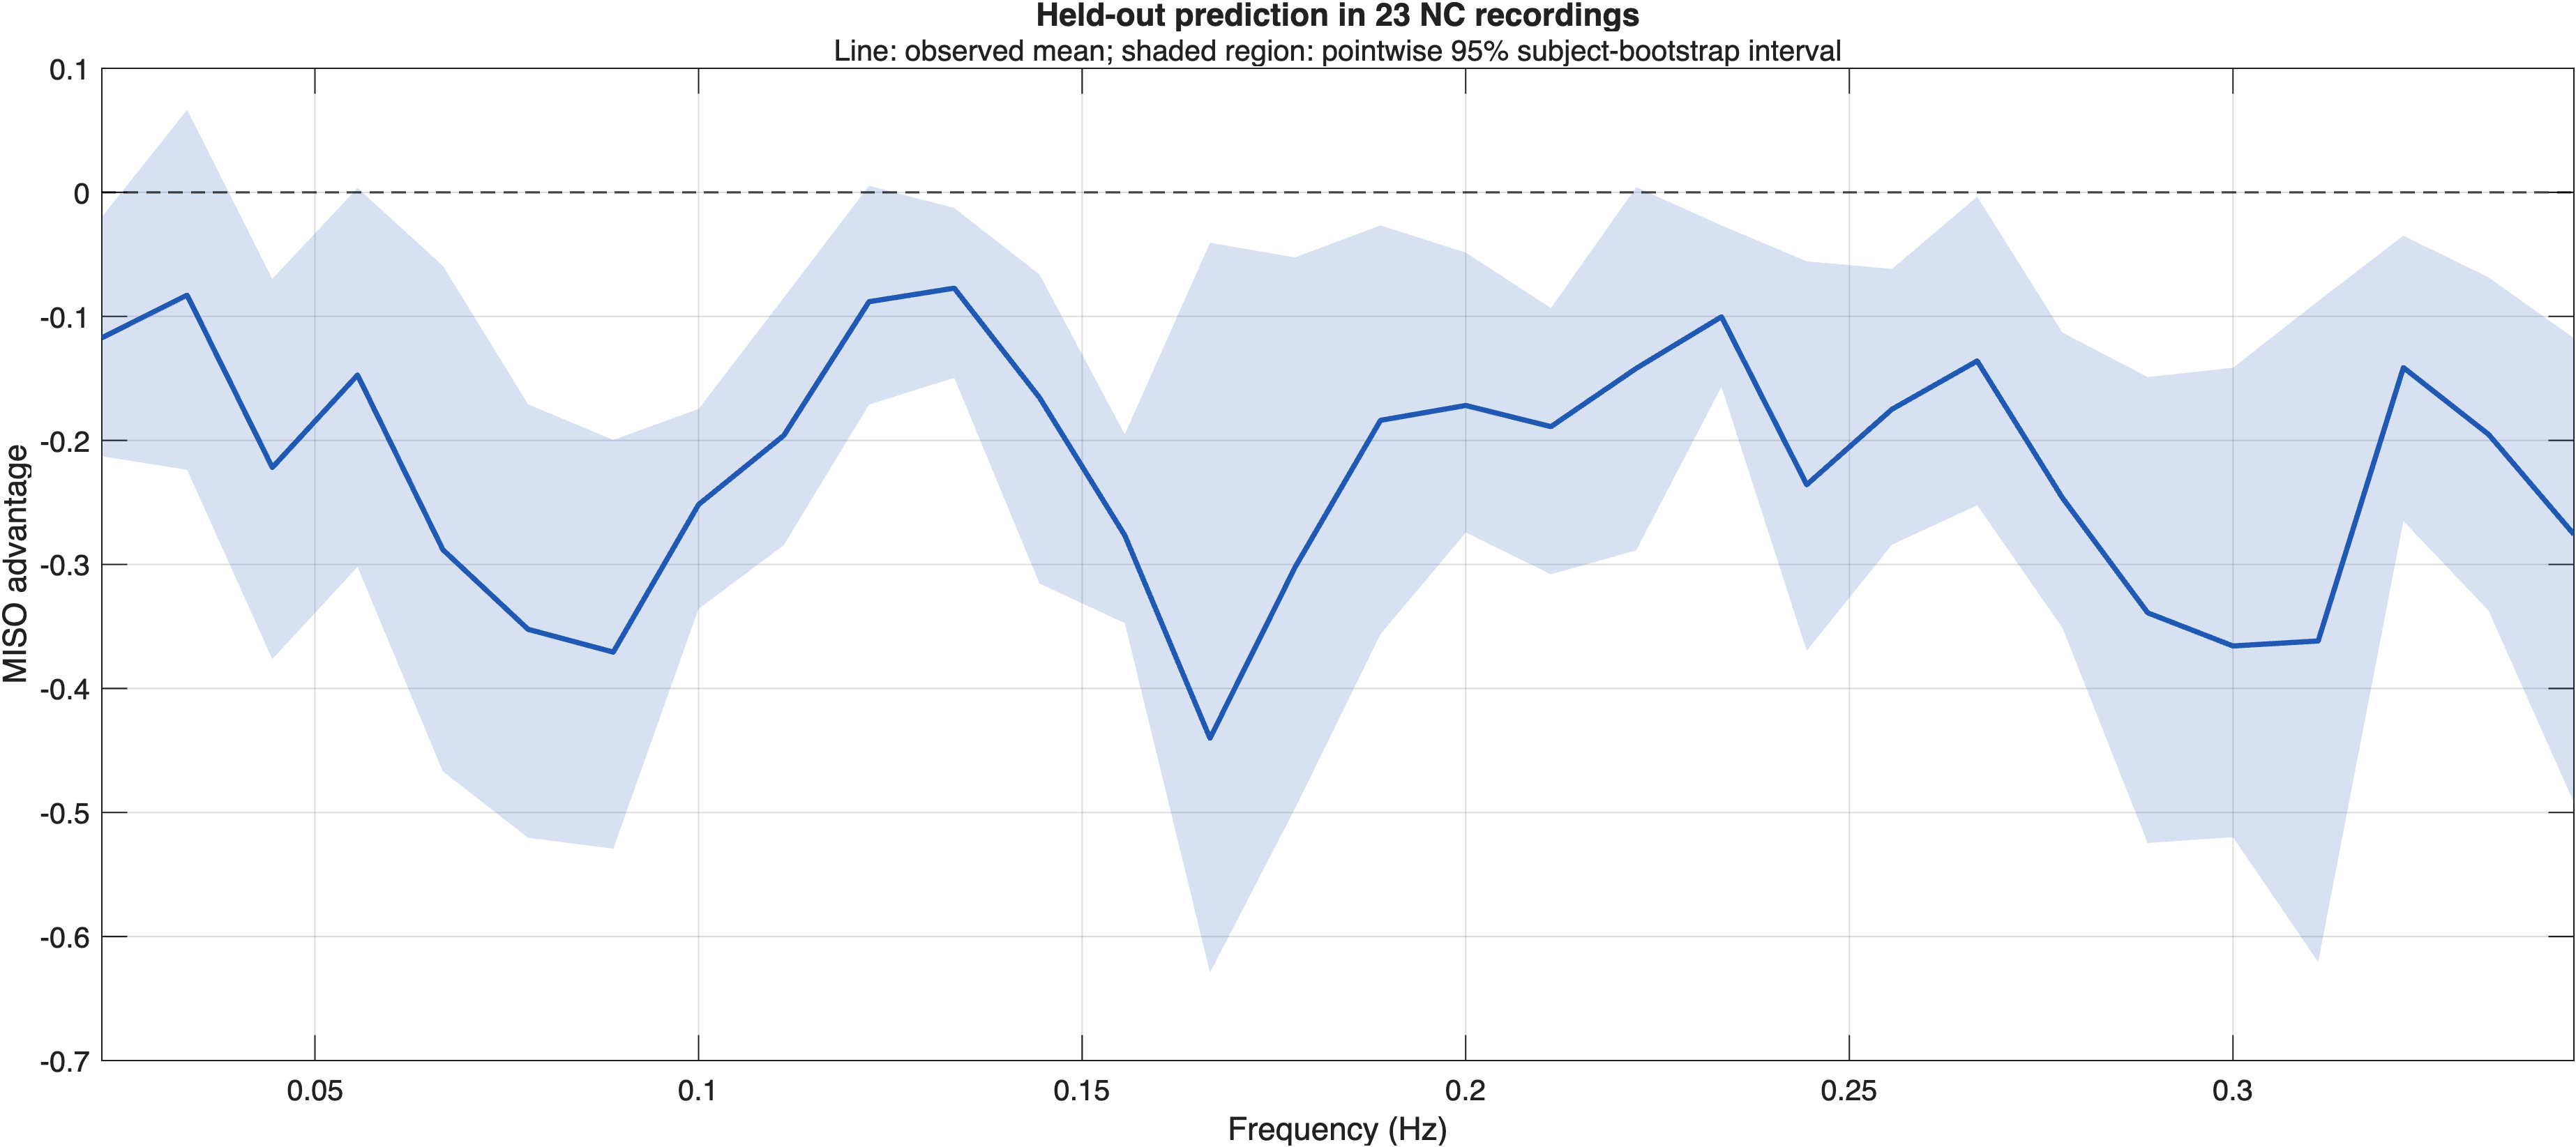
\includegraphics[width=0.92\linewidth]{figure5_nc_validation.png}
    \caption{Held-out CBFV prediction in \NCSubjectCount{} NC recordings.
    The line is the mean within-subject MISO advantage and the shaded region is
    the pointwise 95\% subject-bootstrap interval. Negative values indicate
    lower prediction error with MAP-only SISO; positive values indicate lower
    prediction error with MISO.}
    \label{fig:nc}
\end{figure}

\begin{thebibliography}{99}

\bibitem{Panerai2023}
Panerai RB, Brassard P, Burma JS, et al.; Cerebrovascular Research Network.
Transfer function analysis of dynamic cerebral autoregulation: a CARNet white
paper 2022 update. \textit{J Cereb Blood Flow Metab}. 2023;43(1):3--25.
doi:10.1177/0271678X221119760.

\bibitem{Hoiland2019}
Hoiland RL, Fisher JA, Ainslie PN. Regulation of the cerebral circulation by
arterial carbon dioxide. \textit{Compr Physiol}. 2019;9(3):1101--1154.
doi:10.1002/cphy.c180021.

\bibitem{Panerai2000}
Panerai RB, Simpson DM, Deverson ST, Mahony P, Hayes P, Evans DH.
Multivariate dynamic analysis of cerebral blood flow regulation in humans.
\textit{IEEE Trans Biomed Eng}. 2000;47(3):419--423.
doi:10.1109/10.827312.

\bibitem{Peng2008}
Peng T, Rowley AB, Ainslie PN, Poulin MJ, Payne SJ. Multivariate system
identification for cerebral autoregulation. \textit{Ann Biomed Eng}.
2008;36(2):308--320. doi:10.1007/s10439-007-9412-9.

\bibitem{Westwick2006}
Westwick DT, Pohlmeyer EA, Solla SA, Miller LE, Perreault EJ.
Identification of multiple-input systems with highly coupled inputs:
application to EMG prediction from multiple intracortical electrodes.
\textit{Neural Comput}. 2006;18(2):329--355.
doi:10.1162/089976606775093855.

\bibitem{Chertoff2020}
Chertoff ME, Billinger SA, Perdomo SJ, Witte E, Ward JL, Alwatban M.
A novel nonlinear system identification for cerebral autoregulation in human:
computer simulation and validation. \textit{Ann Biomed Eng}.
2020;48(4):1207--1217. doi:10.1007/s10439-019-02442-7.

\bibitem{Welch1967}
Welch PD. The use of fast Fourier transform for the estimation of power
spectra: a method based on time averaging over short, modified periodograms.
\textit{IEEE Trans Audio Electroacoust}. 1967;15(2):70--73.
doi:10.1109/TAU.1967.1161901.

\end{thebibliography}

\end{document}
